\documentclass[twoside,letterpaper]{refrep}
\usepackage{makeidx}
\usepackage{natbib}
\usepackage{xspace}
\usepackage{graphicx}
\usepackage{verbatim}
\usepackage{threeparttable}

\settextfraction{1.0}

\newcommand{\facversion}{{0.7.9}\xspace}
\newcommand{\opt}[1]{
  {\textnormal{[}}{#1}\hspace{0.5mm}{\textnormal{]}}}
\newcommand{\var}[1]{\textit{#1}}
\newcommand{\key}[1]{\texttt{#1}}
\newcommand{\mod}[1]{\texttt{#1}}
\newcommand{\atom}[1]{\textbf{\texttt{#1}}}

\newcommand{\threej}[6]{\ensuremath{\left({#1\atop #4}{#2\atop #5}
{#3\atop #6}\right)}}
\newcommand{\sixj}[6]{\ensuremath{\left\{{#1\atop #4}{#2\atop #5}
{#3\atop #6}\right\}}}

\newenvironment{ttscript}[1]{
	\begin{list}{}{
	\settowidth{\labelwidth}{\texttt{#1}}
	\setlength{\leftmargin}{\labelwidth}
	\addtolength{\leftmargin}{\labelsep}
	\setlength{\parsep}{0.5ex plus0.2ex minus0.2ex}
	\setlength{\itemsep}{0.3ex}
	\renewcommand{\makelabel}[1]{\texttt{##1\hfill}}}}
	{\end{list}}
\newenvironment{dbdesc}{\textbf{Field Description:} \begin{list}
	{:}{\setlength{\labelwidth}{2in}
	   \setlength{\leftmargin}{2in}
	   \setlength{\labelsep}{0.1in}
	   \setlength{\rightmargin}{0.2in}}}
	{\end{list}}
\newenvironment{fundesc}[2]{
	\addcontentsline{toc}{subsubsection}{#1}
	\index{#1}
	\begin{center}
	\begin{minipage}{\textwidth}
	\key{\textbf{#1}}(\var{#2}):\\}
	{\end{minipage}\end{center}}
\newenvironment{vardesc}[1]{
	\addcontentsline{toc}{subsubsection}{#1}
	\index{#1}
	\begin{center}
	\begin{minipage}{\textwidth}
	\key{\textbf{#1}}:\\}
	{\end{minipage}\end{center}}

\newcounter{faq}[section]
\newcommand{\faq}[2]{\stepcounter{faq}
	\begin{minipage}{\textwidth}
	\textbf{Q\arabic{faq}: #1?}\\#2
	\end{minipage}}

\setcounter{tocdepth}{3}

\makeindex

\begin{document}

\title{FAC \facversion Manual}
\author{M. F. Gu\thanks{Chandra Fellow,  mfgu@space.mit.edu} \\
Center for Space Research, MIT \\ Cambridge, MA 02139}

\date{}

\maketitle

\tableofcontents

\chapter{Overview}
\label{cha:overview}

\section{What Is FAC}
FAC stands for The Flexible Atomic Code (and nothing else). It is an
integrated software package to calculate various atomic radiative and
collisional processes, including energy levels, radiative transition rates,
collisional excitation and 
ionization by electron impact, photoionization, autoionization, radiative
recombination and dielectronic capture. The package also includes a
collisional radiative model to construct synthetic spectra for plasmas under
different physical conditions. The various parts of FAC and their
interactions are shown in Figure \ref{fig:flow}. 

\begin{figure}
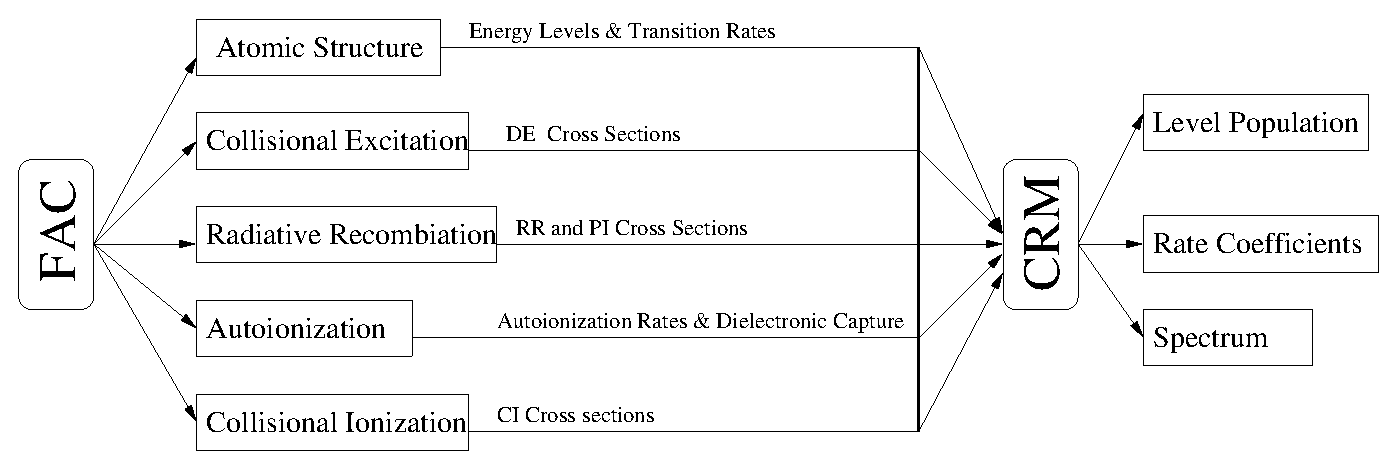
\includegraphics[width=6in]{flow.eps}
\caption{\label{fig:flow}The overview of FAC package.}
\end{figure}

The atomic structure calculation in FAC is based on the relativistic
configuration interaction with independent particle basis wavefunctions. These
basis wavefunctions are derived from a local central potential, which is
self-consistently determined to represent electronic screening of the nuclear
potential. Relativistic effects are fully taken into account using the Dirac
Coulomb Hamiltonian. Higher order QED effects are presently ignored, which may
limit its accuracy for very high-$Z$ elements. Continuum processes are treated
in the distorted-wave (DW) approximation. Systematic application of the
factorization-interpolation method of \citet{barshalom88} makes the present
code highly efficient for large scale calculations. The details of theoretical
background and computational methods are not discussed in this manual,
instead, they are described in a series of papers which are distributed along
with this package and this manual.

FAC is a step forward to bring detailed atomic model accessable to a wide
community of laboratory and astrophysical plasma diagnostics. Its flexible
interface is designed to be useful even for people without a deep
understanding of the underlying atomic theories. It is also powerful enough
for experieced users to explore the effects of algorithmic choices and
different physical approximations.

FAC is freely distributed in the hope that it will be useful. The author makes
every effort to ensure its correctness. However, he does not guarantee its
fitness to any specific purpose. The author is not responsible for any damage
resulting from the use of this program, including failure to obtain or loss of
tenure. 

\section{Obtain and Install FAC}
\index{Install}
\label{sec:install}
The latest version of FAC is \facversion. It can be obtained from anonymous
\textbf{ftp://space.mit.edu/pub/mfgu/fac/}. I can also send a copy to you
through email. Please request to \textbf{mfgu@space.mit.edu}. It is being
continously developed at present, so please check regularly to get the newest
version.

Much of the FAC package is written in ANSI C and Fortran 77. It should 
therefore work on any platform with a C and Fortran 77 compilers. However, 
this is only true to the rather simple command parser come with FAC, referred 
to as SFAC. The flexibility of FAC is realized when the Python interface
(PFAC)is used. The numerical subroutines implemented in FAC are exported
through several Python modules. The computation task can therefore be
completed by programming in the scripting language Python. These python
modules are compiled as shared objects, and are dynamically loaded. This
primarily works under ELF systems, such as almost all modern Unix and Linux
systems. It has also been tested to work under Mac OS X and Windows (In the
case of Windows, the Unix API emulation by Cygwin is required, which is
available at \textbf{www.cygwin.com}). To fully utilize the strength of  
FAC, it is strongly recommended that Python be installed, which can be obtained
from \textbf{www.python.org}.

In all Unix-like systems with Python installed, the installation of FAC 
uses the \verb|distutil| module comes with Python. To install in the standard 
location, download FAC from the above mentioned ftp site, gunzip and extract 
from the tar-ball, change to the top directory and type 
\begin{verbatim}
    python setup.py install
    python setup.py sfac
\end{verbatim}
where the first command installs the Python package \verb|pfac| which 
contains several Python and extension modules, and the second command
installs the SFAC interface in your \verb|${HOME}/bin|, and places two
excutables, \verb|sfac| and \verb|scrm|, in your \verb|${HOME}/bin|. 
This will install the PFAC modules in the standard Python site-package
directory. If Python was installed as root, this requires the root permission
as well. Alternatively, one may install the PFAC package into a given
directory by running, 
\begin{verbatim}
    python setup.py install --prefix=/my/own/dir
\end{verbatim} 
In order for python to find the installed PFAC modules, one would have to 
define an environment variable PYTHONPATH to point to the directory
\verb|/my/own/dir/lib/python#.#/site-packages|, where \verb|#.#| represents
the Python version. In csh, this requires
\begin{verbatim}
    setenv PYTHONPATH /my/own/dir/lib/python#.#/site-packages
\end{verbatim}
or in bash,
\begin{verbatim}
    PYTHONPATH=/my/own/dir/lib/python#.#/site-packages; export PYTHONPATH
\end{verbatim}

Without Python, one may install the SFAC interface by
\begin{verbatim}
    make sfac
    make install
\end{verbatim}

The system must have a \verb|make| compartible with GNU \verb|make|, even if
\verb|setup.py| is used, since this script calls \verb|make| to compile the
libraries. One should check out the README file in the top directory of FAC 
distribution for more instructions.

\section{Quick Start}
\label{sec:start}
\subsection{SFAC Interface}
The SFAC interface is basically a stripped down command interpreter modeled
after Python syntax, with the omission of flow control freatures, such as
conditional execution and loops. Therefore simple Python scripts may be
converted to SFAC input files without difficulty. The Python interface
actually contains functions to do the convertion automatically. Through out
this manuall, we mainly focus on the more useful Python interface. Most of the
Python fuctions implemented in the extension modules are also available in
SFAC interface with identical calling sequences. To use SFAC, one passes the
input files to the two executables \verb|sfac| and \verb|scrm| on the command
line such as 
\begin{verbatim}
    sfac input.sf
    scrm input.sf
\end{verbatim}
or, one may invoke \verb|sfac| and \verb|scrm| without arguments, in which
case, they read from \verb|stdin| for inputs, where commands are interpreted
line by line. The program \verb|sfac| handles atomic calculations, while
\verb|scrm| is used to construct collisional radiative spectral models.

\subsection{PFAC Interface}
To use the PFAC interface, one needs to be familiar with the basics of Python
scripting language. Python has excellent documentations come with the standard
distribution. It is an extremely well designed language to learn, and to use.

Perhaps, the quickest way to get familiar with FAC is to inspect the simple
demo scripts in the \verb|demo/| directory comes with FAC distribution. There
are individual scripts and their SFAC conterparts demonstrating the
calculation of energy levels, radiative transition rates, collisional
excitation and ionization cross sections, radiative recombination cross
sections and autoionization rates. There is also a more advanced example for
the calculation of iron L-shell atomic data, and their application in the
collisional radiative model.

In this section, we look into the details of one of these scripts,
\verb|demo/structure/fe17_structure.py| for the calculation of Ne-like iron
energy levels and radiative transition rates between $n = 2$ and $n = 3$
complexes. The following is a duplication of that script.
\begin{verbatim}
 1: from pfac import fac

 2: fac.SetAtom('Fe')
 3: # 1s shell is closed
 4: fac.Closed('1s')
 5: fac.Config('2*8', group = 'n2')
 6: fac.Config('2*7 3*1', group = 'n3')

 7: # Self-consistent iteration for optimized central potential
 8: fac.ConfigEnergy(0)
 9: fac.OptimizeRadial(['n2', 'n3'])
10: fac.ConfigEnergy(1)
11: fac.Structure('ne.lev.b', ['n2', 'n3'])
12: fac.MemENTable('ne.lev.b')
13: fac.PrintTable('ne.lev.b', 'ne.lev', 1)

14: fac.TransitionTable('ne.tr.b', ['n2'], ['n3'])
15: fac.PrintTable('ne.tr.b', 'ne.tr', 1)
\end{verbatim}
Line numbers are added for easy reference, they are not part of the script. 
As is evident from the above list, all functions implemented in the FAC
extension modules have a naming convention of concatenated capitalized words.
Line 1 imports the extension module \verb|fac| from the package \verb|pfac|.
Alternatively, one could have used
\begin{verbatim}
    from pfac.fac import *
\end{verbatim}
then, all module qualifiers \verb|fac.| in the following lines can be omitted.
Line 2 set the atomic element to be iron. Line 3 is a comment, which starts
with a \verb|#|. Line 4--6 specifies the electronic configurations to be
included in the calculation. The closed shells specified by the function
\verb|Closed| must be inactive in this calculation. In the \verb|Config|
functions, \verb|2*8| stands for an $n = 2$ complexes with 8 electrons, while
\verb|2*7 3*1| stands for all configurations resulting from excitation of one
electron from $n = 2$ to $n = 3$. For more possibilities in the specification
of electronic configurations, one is referred to Chapter \ref{cha:function}.
Line 8--10 carries out a Dirac-Fock-Slater self-consistent calculation to
derive a local central potential which represents the electronic screening of
the nuclear potential. In this calculation, the potential is optimized to the
average electron clouds of configurations \verb|n2| and \verb|n3|, since in
FAC, all atomic processes are treated with basis wavefunctions generated from
a single potential. This
results in the potential to be less optimized for \verb|n2| and \verb|n3|
individually. Lines 8 and 10 are used to make a crude correction to the
resulting energy levels due to this effect. The first call to
\verb|ConfigEnergy(0)| will make individual optimization to all configuration
groups. The average energy of each configuration group is then calculated and
stored under the potentials optimized for that group. The
second call to \verb|ConfigEnergy(1)| will then recalculate the average energy
of configuration groups under the potential taking into account all
configuration groups. The difference between the two represents the effect of
a less optimized potential, and are used to adjust the final energy levels. If
this procedure is not needed, one can omit line 8 and 10 in this script. Line
11 sets up the Hamiltonian matrix for levels in $n = 2$ and $n = 3$ complexes,
diagonalize it, and saves to the energy level information in the binary file
\verb|ne.lev.b|. Line 12 builds an in-memory table of energy levels, which is
used to convert the binary files to their ASCII counterparts in verbose mode,
such as done in Line 13, which converts \verb|ne.lev.b| to \verb|ne.lev| (the
last argument to \verb|PrintTable| indicates it be done in verbose mode). For
the conversion in simple mode (the last argument is 0), the in-memory table is
not needed, and Line 12 may be omitted. For the difference between the verbose
and simple ASCII files, see Chapter \ref{cha:format}. Line 14 calculates the
E1 oscillator strength and transition rates between cofiguration groups
\verb|n2| and \verb|n3|, and saves the results in the binary file
\verb|ne.tr.b|. The function \verb|TransitionTable| accepts an optional 4th
integer argument specifying the transition type. A negative integer means
electric multipol and a positive integer for magnetic multipole. The absolute
value of the integer indicates the rank of the multipole. Therefore, $-1$ would
be E1, $+1$ would be M1, etc. Without this argument, the default is E1, as is
done here. Line 15 converts the binary output to an ASCII file in verbose
mode. The exact formats of binary and ASCII files are explained in Chapter
\ref{cha:format}. Here we list the two ASCII files \verb|ne.lev| and
\verb|ne.tr| resulted from this calculation. 
\begin{verbatim}
File ne.lev:

FAC 0.7.6
Endian	= 0
TSess	= 1029027579
Type	= 1
Verbose	= 1
Fe Z	=  26.0
NBlocks	= 1
E0	= 0, -3.12494784E+04

NELE	= 10
NLEV	= 37
         Energy       P VNL 2J
    0  0.00000000E+00 0 201  0 1*2 2*8      2p6       2p+4(0)0 
    1  7.24353943E+02 1 300  4 1*2 2*7 3*1  2p5 3s1   2p+3(3)3 3s+1(1)4 
    2  7.26393494E+02 1 300  2 1*2 2*7 3*1  2p5 3s1   2p+3(3)3 3s+1(1)2 
    3  7.37238831E+02 1 300  0 1*2 2*7 3*1  2p5 3s1   2p-1(1)1 3s+1(1)0 
    4  7.38577454E+02 1 300  2 1*2 2*7 3*1  2p5 3s1   2p-1(1)1 3s+1(1)2 
    5  7.54684448E+02 0 301  2 1*2 2*7 3*1  2p5 3p1   2p+3(3)3 3p-1(1)2 
    6  7.58348267E+02 0 301  4 1*2 2*7 3*1  2p5 3p1   2p+3(3)3 3p-1(1)4 
    7  7.59979248E+02 0 301  6 1*2 2*7 3*1  2p5 3p1   2p+3(3)3 3p+1(3)6 
    8  7.61135193E+02 0 301  2 1*2 2*7 3*1  2p5 3p1   2p+3(3)3 3p+1(3)2 
    9  7.62972046E+02 0 301  4 1*2 2*7 3*1  2p5 3p1   2p+3(3)3 3p+1(3)4 
   10  7.68711975E+02 0 301  0 1*2 2*7 3*1  2p5 3p1   2p+3(3)3 3p+1(3)0 
   11  7.70705017E+02 0 301  2 1*2 2*7 3*1  2p5 3p1   2p-1(1)1 3p-1(1)2 
   12  7.73933716E+02 0 301  2 1*2 2*7 3*1  2p5 3p1   2p-1(1)1 3p+1(3)2 
   13  7.74405396E+02 0 301  4 1*2 2*7 3*1  2p5 3p1   2p-1(1)1 3p+1(3)4 
   14  7.91043762E+02 0 301  0 1*2 2*7 3*1  2p5 3p1   2p-1(1)1 3p-1(1)0 
   15  8.00673401E+02 1 302  0 1*2 2*7 3*1  2p5 3d1   2p+3(3)3 3d-1(3)0 
   16  8.01713074E+02 1 302  2 1*2 2*7 3*1  2p5 3d1   2p+3(3)3 3d-1(3)2 
   17  8.03623108E+02 1 302  4 1*2 2*7 3*1  2p5 3d1   2p+3(3)3 3d+1(5)4 
   18  8.03792480E+02 1 302  8 1*2 2*7 3*1  2p5 3d1   2p+3(3)3 3d+1(5)8 
   19  8.04533203E+02 1 302  6 1*2 2*7 3*1  2p5 3d1   2p+3(3)3 3d-1(3)6 
   20  8.06197388E+02 1 302  4 1*2 2*7 3*1  2p5 3d1   2p+3(3)3 3d-1(3)4 
   21  8.07330078E+02 1 302  6 1*2 2*7 3*1  2p5 3d1   2p+3(3)3 3d+1(5)6 
   22  8.12196411E+02 1 302  2 1*2 2*7 3*1  2p5 3d1   2p+3(3)3 3d+1(5)2 
   23  8.17411499E+02 1 302  4 1*2 2*7 3*1  2p5 3d1   2p-1(1)1 3d-1(3)4 
   24  8.18119019E+02 1 302  4 1*2 2*7 3*1  2p5 3d1   2p-1(1)1 3d+1(5)4 
   25  8.18746826E+02 1 302  6 1*2 2*7 3*1  2p5 3d1   2p-1(1)1 3d+1(5)6 
   26  8.26612610E+02 1 302  2 1*2 2*7 3*1  2p5 3d1   2p-1(1)1 3d-1(3)2 
   27  8.61517029E+02 0 300  2 1*2 2*7 3*1  2s1 3s1   2s+1(1)1 3s+1(1)2 
   28  8.68436157E+02 0 300  0 1*2 2*7 3*1  2s1 3s1   2s+1(1)1 3s+1(1)0 
   29  8.94455078E+02 1 301  0 1*2 2*7 3*1  2s1 3p1   2s+1(1)1 3p-1(1)0 
   30  8.94953308E+02 1 301  2 1*2 2*7 3*1  2s1 3p1   2s+1(1)1 3p-1(1)2 
   31  8.97325012E+02 1 301  4 1*2 2*7 3*1  2s1 3p1   2s+1(1)1 3p+1(3)4 
   32  8.99311401E+02 1 301  2 1*2 2*7 3*1  2s1 3p1   2s+1(1)1 3p+1(3)2 
   33  9.39470825E+02 0 302  2 1*2 2*7 3*1  2s1 3d1   2s+1(1)1 3d-1(3)2 
   34  9.39646851E+02 0 302  4 1*2 2*7 3*1  2s1 3d1   2s+1(1)1 3d-1(3)4 
   35  9.39932495E+02 0 302  6 1*2 2*7 3*1  2s1 3d1   2s+1(1)1 3d+1(5)6 
   36  9.44828674E+02 0 302  4 1*2 2*7 3*1  2s1 3d1   2s+1(1)1 3d+1(5)4 


File ne.tr:

FAC 0.7.6
Endian	= 0
TSess	= 1020438482
Type	= 2
Verbose	= 1
Fe Z	= 26.0
NBlocks	= 1

NELE	= 10
NTRANS	= 7
Multip	= -1
Gauge	= 2
Mode	= 1
    2	 2	    0	 0	 7.2639E+02  1.22460954E-01  9.34608241E+11
    4	 2	    0	 0	 7.3858E+02  1.04401819E-01  8.23736467E+11
   16	 2	    0	 0	 8.0171E+02  1.02572953E-02  9.53583862E+10
   22	 2	    0	 0	 8.1220E+02  6.31992579E-01  6.03006697E+12
   26	 2	    0	 0	 8.2661E+02  2.61516809E+00  2.58459031E+13
   30	 2	    0	 0	 8.9495E+02  3.35455649E-02  3.88618945E+11
   32	 2	    0	 0	 8.9931E+02  2.80109644E-01  3.27669724E+12
\end{verbatim}

In file \verb|ne.lev|, the energy, parity, $2J$ ($J$ is the total
angular momentum of the level), and configuration coupling informations are
listed. In file \verb|ne.tr|, the upper and lower level indexes, the $2J$
values of these levels, the transition energy, $gf$-values, and radiative
decay rates are given.

\section*{Acknowledgments}
Throughout the development of this work, the discussion with Ehud Behar, Masao
Sako, Peter Beiersdorfer, Ali Kinkhabwala and Steven Kahn has been very
useful. Many Fortran 77 subroutines were retrieved from Netlib repository
(\textbf{www.netlib.org}) and used in this package, as well as several
programs from Computer Physics Communications Program Library at
\textbf{www.cpc.cs.qub.ac.uk}. The multi-precision floating point arithmetic
package used here is developed by \citet{bailey93} of NASA Ames Research
Center.

This work is supported by NASA through Chandra Postdoctoral Fellowship Award
Number PF01-10014 issued by the Chandra X-ray Observatory Center, which is
operated by Smithsonian Astrophysical Observatory for and on behalf of NASA
under contract NAS8-39073. 

Any opinions, findings and conclusions or
recommendations expressed in this manual are those of the author and do not
necessrarily reflect the views of the National Aeronautics Space
Administration and/or the Smithonian Astrophysical Observatory.

\chapter{Description of Output Files}
\label{cha:format}
The primary output files of FAC are in binary format. The I/O functionality
and the conversion from binary to ASCII format are implemented in the source
files \verb|faclib/dbase.h| and \verb|faclib/dbase.c|. In this chapter, we
describe the structure of these files in detail.

\section{Binary Format}
\label{sec:binary}
\index{Binary format}
Presently, FAC produces 8 different types of files. Each type is asigned
a unique integer from 1--8, which corresponds to a macro define in the file
\verb|faclib/dbase.h|. These types are
\begin{description}
\item[\texttt{DB\_EN = 1}] Energy levels produced by the function
\verb|fac.Structure|. 
\item[\texttt{DB\_TR = 2}] Radiative transition rates produced by
\verb|fac.TransitionTable|.
\item[\texttt{DB\_CE = 3}] Collisional excitation cross sections produced by
\verb|fac.CETable|. 
\item[\texttt{DB\_RR = 4}] Radiative recombination and photoionization cross
sections produced by \verb|fac.RRTable|.
\item[\texttt{DB\_AI = 5}] Autoionization rates produced by \verb|fac.AITable|.
\item[\texttt{DB\_CI = 6}] Collisional ionization cross sections produced by
\verb|fac.CITable|. 
\item[\texttt{DB\_SP = 7}] Spectral line strengths produced by
\verb|crm.SpecTable|. 
\item[\texttt{DB\_RT = 8}] Various population rates produced by
\verb|crm.RateTable|. 
\end{description}

All files have a common structure. It consists of a file header and one or
more data blocks. Each data block is comprised of a data header and one or
more data records. In the following, we show the C definition of all structs
and describe each field in detail. When one field is a pointer, it means that
an array is saved in the database. The pointer points to the memory location
where the data is stored. The value of the pointer itself is also
saved in the file followed by the data stored in the array. Obviously, the
saved pointer itself has no meaning once the program exits (since it is a
memory location), it is saved for the sake of convenience. When reading out
the data from the database file, these pointer values should be ignored.

\subsection{\texttt{F\_HEADER}}
\index{F\_HEADER}
\texttt{F\_HEADER} is the file header common to all data files. 

\begin{verbatim}
typedef struct _F_HEADER_ {
  long  tsession;
  int   version;
  int   sversion;
  int   ssversion;
  int   type;
  float atom;
  char  symbol[4];
  int   nblocks;
} F_HEADER;
\end{verbatim}

\begin{dbdesc}
\item[\texttt{long tsession}:] Time stamp when the file is created. This is the
value returned by the C lib function time(0). It is platform dependent. 
\item[\texttt{int version}:] Major version number of FAC.
\item[\texttt{int sversion}:] Minor version number of FAC.
\item[\texttt{int ssversion}:] Release number of FAC.
\item[\texttt{int type}:] Type of the data file. An integer from 1--8.
\item[\texttt{float atom}:] Atomic number.
\item[\texttt{char symbol[4]}:] The first 3 bytes contains a NULL
terminated C string representing the 2-charactor abbr. of atomic symbol. The
4th byte is either 0 or 1, indicating whether the platform stores data in
liitle or big endian.
\item[\texttt{int nblocks}:] Number of data blocks in this file.
\end{dbdesc}

\subsection{\texttt{EN\_HEADER}}
\index{EN\_HEADER}
\texttt{EN\_HEADER} is the data header for energy level data blocks.

\begin{verbatim}
typedef struct _EN_HEADER_ {
  long position;
  long length;
  int nele;
  int nlevels;
} EN_HEADER;
\end{verbatim}

\begin{dbdesc}
\item[\texttt{long position}:] The number of bytes from the beginning of the
file to the place where this data block starts.
\item[\texttt{long length}:] Number of bytes in this data block, excluding the
length of the header.
\item[\texttt{int nele}:] Number of electrons in the ion for this block.
\item[\texttt{int nlevels}:] Number of levels in this block.
\end{dbdesc}

\subsection{\texttt{EN\_RECORD}}
\index{EN\_RECORD}
\texttt{EN\_RECORD} represents an energy level.

\begin{verbatim}
#define LNCOMPLEX   32
#define LSNAME      24
#define LNAME       56

typedef struct _EN_RECORD_ {
  short p;
  short j;
  int ilev;
  float energy;
  char ncomplex[LNCOMPLEX];
  char sname[LSNAME];
  char name[LNAME];
} EN_RECORD;
\end{verbatim}

\begin{dbdesc}
\item[\texttt{LNCOMPLEX}:] The length of array holding the complex name.
\item[\texttt{LSNAME}:] The length of array holding the non-relativistic
configuration name.
\item[\texttt{LNAME}:] The length of array holding the relativistic
configuration array.
\item[\texttt{short p}:] The parity of the level. This parameter was changed
in version 0.7.6, and it becomes $\pm(100\times n + l)$, where $n$ and $l$ are
the principal quantum number and orbital angular number of the valence
electron, and the $\pm$ sign indicates an even ($+$) or odd ($-$) parity state.
\item[\texttt{short j}:] 2 $\times$ the total angular momentum of the level.
\item[\texttt{int ilev}:] The index of the level.
\item[\texttt{energy}:] The energy of the level in Hartree.
\item[\texttt{char ncomplex[LNCOMPLEX]}:] The complex name. It is in the format
of \verb|n1*nq1 n2*nq2|$\cdots$, where \verb|n1| and \verb|n2| are the
principal quantum numbers of the shell, \verb|nq1| and \verb|nq2| are the
occupation number of these shells.
\item[\texttt{char sname[LSNAME]}:] The non-relativstic configuration name of
the level. Each non-relativistic shell is denoted by the standard
spectroscopic notation, e.g., \verb|2p2| for 2 electrons in $2p$ shell. Only
open and non-empty shells are given. No coupling information is available in
this name.
\item[\texttt{char name[LNAME]}:] The relativstic configuration name of the
level. Each shell is denoted such that \verb|2p+2(2)| represents 2 electrons in
$2p_{3/2}(J=1)$ and \verb|2p-2(2)| represents 2 electrons in
$2p_{1/2}(J=1)$. The number in the parenthesis is 2 times the total angular
momentum of the coupled shell. Immediately after the parenthesis, there is a
number indicate the $2J$ value when all preceding shells are
coupled. Therefore, \verb|2p+2(2)2 2p-2(2)0| represents a state
$[2p_{3/2}^{2}(J=1) 2p_{1/2}^2(J=1)]J=0$.
\end{dbdesc}

\subsection{\texttt{TR\_HEADER}}
\index{TR\_HEADER}
\texttt{TR\_HEADER} is the data header for the radiative transition data
blocks. 

\begin{verbatim}
typedef struct _TR_HEADER_ {
  long position;
  long length;
  int nele;
  int ntransitions;
  int gauge;
  int mode;
  int multipole;
} TR_HEADER;
\end{verbatim}

\begin{dbdesc}
\item[\texttt{long position}:] The number of bytes from the beginning of the
file to the place where this data block starts.
\item[\texttt{long length}:] Number of bytes in this data block, excluding the
length of the header.
\item[\texttt{int nele}:] Number of electrons in the ion for this block.
\item[\texttt{int ntransitions}:] Number of transitions in this block.
\item[\texttt{int gauge}:] Gauge used in the calculation. 1 is Coulomb gauge, or
the velocity form in non-relativistic limit. 2 is Babushkin gauge or the
length form.
\item[\texttt{int mode}:] Mode used in the calculation. 0 is fully
relativistic. 1 is non-relativistic approximation for multipole operators.
\item[\texttt{int multipole}:] Multipole type of the transition. Its absolute
value is the rank of the multipole, 1 for dipole, 2 for quadrupole, etc. The
positive sign for magnetic type and negative sign for electric type.
\end{dbdesc}

\subsection{\texttt{TR\_RECORD}}
\index{TR\_RECORD}
\texttt{TR\_RECORD} is the for radiative transition data.

\begin{verbatim}
typedef struct _TR_RECORD_ {
  int lower;
  int upper;
  float strength;
} TR_RECORD;
\end{verbatim}

\begin{dbdesc}
\item[\texttt{int lower}:] The lower level index of the transition.
\item[\texttt{int upper}:] The upper level index of the transition.
\item[\texttt{float strength}:] The weighted oscillator strength $gf$ of the
transition. The weighted radiative transition rate is related to $gf$ as (in
atomic units):
\begin{equation}
gA = 2\alpha^3 \omega^2 gf,
\end{equation}
where $\alpha$ is the fine structure constant, and $\omega$ is transition
energy in Hartree atomic units. 

\end{dbdesc}

\subsection{\texttt{CE\_HEADER}}
\index{CE\_HEADER}
\texttt{CE\_HEADER} is the data header for collisional excitation data blocks.

\begin{verbatim}
typedef struct _CE_HEADER_ {
  long position;
  long length;
  int nele;
  int ntransitions;
  int qk_mode;
  int n_tegrid;
  int n_egrid;
  int egrid_type;
  int n_usr;
  int usr_egrid_type;
  int nparams;
  int pw_type;
  int msub;
  float te0;
  double *tegrid;
  double *egrid;
  double *usr_egrid;
} CE_HEADER;
\end{verbatim}

\begin{dbdesc}
\item[\texttt{long position}:] The number of bytes from the beginning of the
file to the place where this data block starts.
\item[\texttt{long length}:] Number of bytes in this data block, excluding the
length of the header.
\item[\texttt{int nele}:] Number of electrons in the ion for this block.
\item[\texttt{int ntransitions}:] Number of transitions in this block.
\item[\texttt{int qk\_mode}:] The mode for the calculation of radial
integrals. There are 3 choices for collisional excitation. 0 for EXACT, 1 for
INTERPOLATE, and 2 for FIT. In the EXACT mode, the collison strengths are
calculated at the energy grid specified as is, so the \texttt{egrid} and
\texttt{usr\_egrid} must be the same. In the INTERPOLATE mode, the collision
strengths are calculated at \texttt{egrid}, and interpolated to
\texttt{usr\_egrid}. In the FIT mode, the collision strengths are fitted to an
analytic formula and the parameters are output as well. For collision
strengths of magnetic sublevels, the FIT mode is not implemented.
\item[\texttt{int n\_tegrid}:] Number of points for the transition energy grid.
\item[\texttt{int n\_egrid}:] Number of points for the collision energy grid.
\item[\texttt{int egrid\_type}:] Type of the energy grid. 0 for the incident
electron energy, 1 for scattered electron energy.
\item[\texttt{int n\_usr}:]N umber of points for the user collision energy
grid.
\item[\texttt{int usr\_egrid\_type}:] Type of the user energy grid. 0 for the
incident electron energy, 1 for scattered electron energy.
\item[\texttt{int nparams}:] Number of parameters in the fitting formula if the
collision strengths are calculated in the FIT mode. At present,
\texttt{nparams} is 4. 
\item[\texttt{int pw\_type}:] Partial wave type for the last summation. 0 for
the incident electron, 1 for the scattered electron.
\item[\texttt{int msub}:] 0 for total collision strength, 1 for magnetic
sublevel specific collision strength.
\item[\texttt{float te0}:] The characteristic transition energy of the 
transition array. This is used for the automatic construction of the 
collision energy grid. The grid has equal space in $\ln$(\texttt{egrid+te0})
if \texttt{egrid\_type = 1}, otherwise, this variable is not used.
\item[\texttt{double *tegrid}:] The transition energy grid, the number of
elements is given by \texttt{n\_tegrid}.
\item[\texttt{double *egrid}:] The energy grid, the number of elements is
given by \texttt{n\_egrid}.
\item[\texttt{double *usr\_egrid}:] The user energy grid, the number of
elements is given by \texttt{n\_usr}.
\end{dbdesc}

\subsection{\texttt{CE\_RECORD}}
\index{CE\_RECORD}
\texttt{CE\_RECORD} is for collisional excitation data.

\begin{verbatim}
typedef struct _CE_RECORD_ {
  int lower;
  int upper;
  int nsub;
  float bethe[4];
  float *params;
  float *strength;
} CE_RECORD;
\end{verbatim}

\begin{dbdesc}
\item[\texttt{int lower}:] The lower level index.
\item[\texttt{int upper}:] The upper level index.
\item[\texttt{int nsub}:] Number of magnetic sublevel transitions. Because of
time reversal symmetry, $\sigma_{m_1\to m_2}=\sigma_{-m_1\to -m_2}$, only cross
sections with $m_1 <= 0$ are tabulated.
\item[\texttt{float bethe[4]}:] The Bethe coefficients in the first-Born
approximation. If \texttt{bethe[0]}<0, it is a spin forbidden transition,
and all Bethe coefficients are 0.0, i.e., the exchange cross sections are not
calculated in the Born approximation. Otherwise, the high energy behaviour of
the collision strengths are given by
\begin{eqnarray}
x &=& \frac{E_0}{E_{th}} \nonumber\\
\Omega &=& b_0\log(x) + b_1 + \frac{b_2}{x} + \frac{b_3}{x^2},
\end{eqnarray}
where $b_0$, $b_1$, $b_2$, and $b_3$ are the elements of the floating array
\texttt{bethe}. 
\item[\texttt{float *params}:] Parameters for the fitting formula, if the
fitting mode is used. The number of elements is given by \texttt{nparams} in
\texttt{CE\_HEADER}. In the present implementation, different fitting formulae
are used for allowed and forbidden transitions. The number of parameters is 4
in all cases. 

For dipole and higher multipole allowed transitions, the
collision strength $\Omega$ is given by
\begin{eqnarray}
x &=& \frac{E_0}{E_{th}} \nonumber\\
\Omega &=& p_0\left(\frac{1}{x}\right)^{p_1} + 
p_2\left(1-\frac{1}{x}\right)^{p_3} + b\ln x,
\end{eqnarray}
where $E_0$ is the energy of the incident electron, $E_{th}$ is the transition
threshold, $p_0$, $p_1$, $p_2$ and $p_4$ are four parameters, and $b$ is the
Bethe coeffificient, which is 0 for non-dipole transitions.

For forbidden transitions, the collision strength is given by
\begin{eqnarray}
\gamma &=& -2.0 + p_1\frac{1}{p_3+x} + 
p_2\left(\frac{1}{p_3+x}\right)^2\nonumber\\
\Omega &=& p_0x^\gamma.
\end{eqnarray}
\item[\texttt{float *stregnth}:] Collision stregnth on the user energy
grid. The number of elements is given by \texttt{n\_usr} in
\texttt{CE\_HEADER}. It is related to the excitation cross section as (in
atomic units):
\begin{equation}
\sigma = \frac{\pi}{k_0^2g_0}\Omega,
\end{equation}
where $g_0$ is the statistical weight of the initial state, and $k_0$ is the
kinetic momentum of the incident electron. The number of elements in this
array is \texttt{nsub}$\times$\texttt{n\_usr}.
\end{dbdesc}

\subsection{\texttt{RR\_HEADER}}
\index{RR\_HEADER}
\texttt{RR\_HEADER} is the data header for radiative recombination and
photoionization data blocks.

\begin{verbatim}
typedef struct _RR_HEADER_ {
  long position;
  long length;
  int nele;
  int ntransitions;
  int qk_mode;
  int multipole;
  int n_tegrid;
  int n_egrid;
  int egrid_type;
  int n_usr;
  int usr_egrid_type;
  int nparams;
  double *tegrid;
  double *egrid;
  double *usr_egrid;
} RR_HEADER;
\end{verbatim}

\begin{dbdesc}
\item[\texttt{long position}:] The number of bytes from the beginning of the
file to the place where this data block starts.
\item[\texttt{long length}:] Number of bytes in this data block, excluding the
length of the header.
\item[\texttt{int nele}:] Number of electrons in the ion for this block.
\item[\texttt{int ntransitions}:] Number of transitions in this block.
\item[\texttt{int qk\_mode}:] The mode for the calculation of radial
integrals. There are 3 choices at present. 0 for EXACT, 1 for INTERPOLATE, and
2 for FIT, similar to collsional excitation. However, even if the FIT
mode is used, the fitting formula is only valid in the high energy asymptotic
regions. The low energy results should be obtained by interpolation.
\item[\texttt{int multipole}:] Multipole type of the transition. Its absolute
value is the rank of the multipole, 1 for dipole, 2 for quadrupole, etc. The
positive sign for magnetic type and negative sign for electric type. Usually,
only E1 type is relavent for radiative recombination and photoionization.
\item[\texttt{int n\_tegrid}:] Number of points for the transition energy grid.
\item[\texttt{int n\_egrid}:] Number of points for the collision energy grid.
\item[\texttt{int egrid\_type}:] Type of the energy grid. 0 for the incident
photon energy, 1 for photo-electron energy.
\item[\texttt{int n\_usr}:] Number of points for the user collision energy
grid.
\item[\texttt{int usr\_egrid\_type}:] Type of the user energy grid. 0 for the
incident photon energy, 1 for photo-electron energy.
\item[\texttt{int nparams}:] Number of parameters in the fitting formula if the
bound-free oscillator strengths are calculated in the FIT mode. In the present
imprementation, \texttt{nparams} is 4.
\item[\texttt{double *tegrid}:] The transition energy grid, the number of
elements is given by \texttt{n\_tegrid}.
\item[\texttt{double *egrid}:] The energy grid, the number of elements is
given by \texttt{n\_egrid}.
\item[\texttt{double *usr\_egrid}:] The user energy grid, the number of
elements is given by \texttt{n\_usr}.
\end{dbdesc}

\subsection{\texttt{RR\_RECORD}}
\index{RR\_RECORD}
\texttt{RR\_RECORD} is for radiative recombination and photoionization data.

\begin{verbatim}
typedef struct _RR_RECORD_ {
  int b;
  int f;
  int kl;
  float *params;
  float *strength;
} RR_RECORD;
\end{verbatim}

\begin{dbdesc}
\item[\texttt{int b}:] The bound state index.
\item[\texttt{int f}:] The free state index.
\item[\texttt{int kl}:] The orbital angular momentum of the ionized shell for
the dominant wavefunction component.
\item[\texttt{float *params}:] The parameters in the fitting formula for the
bound-free oscillator strength, if the FIT mode is
used. The fitting formula only provides a high energy asymptotic behavior. Low
energy values should be interpolated from the tabulated strengths. The fitting
formula is
\begin{eqnarray}
x &=& \frac{E_e+p_3}{p_3} \nonumber\\
y &=& \frac{1+p_2}{\sqrt{x}+p_2} \nonumber\\
\frac{d(gf)}{dE} &=&
\frac{E_\gamma}{E_e+p_3}p_0x^{-3.5-l+\frac{1}{2}p_1}y^{p_1}, 
\end{eqnarray}
where $E_e$ is the photo-electron energy, $E_\gamma$ is the photon energy,
$E_{th}$ is the ionization threshold, $p_0$, $p_1$, $p_2$, and $p_3$ are the
parameters, and $l$ is the orbital angular momentum of the ionized
shell. The asymptotic behavior represented by the power law only takes into
account the ionization of the dominant basis in the wavefunction
expansion. The result is in atomic unit Hartree$^{-1}$.
\item[\texttt{float *strength}:] The weighted bound-free oscillator strength in
atomic units. It is related to photoionization and radiative recombination as
(in atomic units):
\begin{eqnarray}
\sigma_{PI} &=& 2\pi\alpha\frac{ d f}{ d E} \nonumber\\*
\sigma_{RR} &=& \frac{\alpha^2}{2}\frac{g_i}{g_f}\frac{\omega^2}{\varepsilon}
\sigma_{PI},
\end{eqnarray}
where $\alpha$ is the fine structure constant, $g_i$ and $g_f$ are the
statistical weight of the bound states before and after the photoionzation
takes place respectively, $\omega$ is the photon energy, and $\varepsilon$ is
the energy of the ejected photo-electron. The tabulated values are $d(gf)/dE$.
\end{dbdesc}

\subsection{\texttt{AI\_HEADER}}
\index{AI\_HEADER}
\texttt{AI\_HEADER} is the data header for autoionization data blocks.

\begin{verbatim}
typedef struct _AI_HEADER_ {
  long position;
  long length;
  int nele;
  int ntransitions;
  int channel;
  int n_egrid;
  double *egrid;
} AI_HEADER;
\end{verbatim}

\begin{dbdesc}
\item[\texttt{long position}:] The number of bytes from the beginning of the
file to the place where this data block starts.
\item[\texttt{long length}:] Number of bytes in this data block, excluding the
length of the header.
\item[\texttt{int nele}:] Number of electrons in the ion for this block.
\item[\texttt{int ntransitions}:] Number of transitions in this block.
\item[\texttt{int channel}:] This an identifier to label the autoionization
channel, which does not have specific physical meaning.
\item[\texttt{int n\_egrid}:] The number of points for the Auger electron
energy grid. The autoionzation radial integrals are calculated on this grid
and interpolated to the actual discrete energies.
\item[\texttt{double *egrid}:] The energy grid. The number of elements is
given by \texttt{n\_egrid}.
\end{dbdesc}

\subsection{\texttt{AI\_RECORD}}
\index{AI\_RECORD}
\texttt{AI\_RECORD} is for autoionization data.

\begin{verbatim}
typedef struct _AI_RECORD_ {
  int b;
  int f;
  float rate;
} AI_RECORD;
\end{verbatim}

\begin{dbdesc}
\item[\texttt{int b}:] The bound state index.
\item[\texttt{int f}:] The free state index.
\item[\texttt{float rate}:] The autoionization rate.
\end{dbdesc}

\subsection{\texttt{CI\_HEADER}}
\index{CI\_HEADER}
\texttt{CI\_HEADER} is the data header for collisional ionization data blocks.

\begin{verbatim}
typedef struct _CI_HEADER_ {
  long position;
  long length;
  int nele;
  int ntransitions;
  int qk_mode;
  int n_tegrid;
  int n_egrid;
  int egrid_type;
  int n_usr;
  int usr_egrid_type;
  int nparams;
  int pw_type;
  double *tegrid;
  double *egrid;
  double *usr_egrid;
} CI_HEADER;
\end{verbatim}

\begin{dbdesc}
\item[\texttt{long position}:] The number of bytes from the beginning of the
file to the place where this data block starts.
\item[\texttt{long length}:] Number of bytes in this data block, excluding the
length of the header.
\item[\texttt{int nele}:] Number of electrons in the ion for this block.
\item[\texttt{int ntransitions}:] Number of transitions in this block.
\item[\texttt{int qk\_mode}:] The mode for the calculation of radial
integrals. At present, there are 3 choices. 3 for CB mode (Coulomb-Born), 4
for DW mode (distorted-wave), and 5 for BED mode (binary-encounter-dipole). In
CB mode, the radial integrals are obtained by looking up a table of
Coulomb-Born-Exchange results from \citet{golden77,golden80}, which is very
fast. In DW mode, the integrals are calculated using the distorted-wave
approximation, which is very slow. In BED mode, the binary-encounter-dipole
theory of \citet{kim94} is used which makes use of bound-free oscillator
strength of the same transition. This method is also very fast.
\item[\texttt{int n\_tegrid}:] Number of points for the transition energy grid.
\item[\texttt{int n\_egrid}:] Number of points for the collision energy grid.
\item[\texttt{int egrid\_type}:] Type of the energy grid. 0 for the incident
electron energy, 1 for the total energy of scattered and ejected electron.
\item[\texttt{int n\_usr}:]N umber of points for the user collision energy
grid.
\item[\texttt{int usr\_egrid\_type}:] Type of the user energy grid. 0 for the
incident electron energy, 1 for the total energy of scattered and ejected
electrons .
\item[\texttt{int nparams}:] Number of parameters in the fitting formula. The
final collision strength for total ionization cross sections are fitted with a
4 parameter formula.
\item[\texttt{int pw\_type}:] Partial wave type for the last summation. 0 for
the incident electron, 1 for the scattered electron. It is always 0 for
distorted-wave calculation of ionization.
\item[\texttt{double *tegrid}:] The transition energy grid, the number of
elements is given by \texttt{n\_tegrid}.
\item[\texttt{double *egrid}:] The energy grid, the number of elements is
given by \texttt{n\_egrid}.
\item[\texttt{double *usr\_egrid}:] The user energy grid, the number of
elements is given by \texttt{n\_usr}.
\end{dbdesc}

\subsection{\texttt{CI\_RECORD}}
\index{CI\_RECORD}
\texttt{CI\_RECORD} is for collisional ionization data.

\begin{verbatim}
typedef struct _CI_RECORD_ {
  int b;
  int f;
  int kl;
  float *params;
  float *strength;
} CI_RECORD;
\end{verbatim}

\begin{dbdesc}
\item[\texttt{int b}:] The bound state index.
\item[\texttt{int f}:] The free state index.
\item[\texttt{int kl}:] The orbital angular momentum of the ionized shell for
the dominant wavefunction component.
\item[\texttt{float *params}:] The parameters in the fitting formula for the
collision strength. The number of elements is given by \texttt{nparams} in
\texttt{CI\_HEADER}, which is 4. The formula used is
\begin{eqnarray}
x &=& \frac{E_0}{E_{th}} \nonumber\\
y &=& 1-\frac{1}{x} \nonumber\\
\Omega &=& p_0\ln x + p_1y^2 + p_2\frac{1}{x}y + p_3\frac{1}{x^2}y,
\end{eqnarray}
where $E_0$ is the energy of the incident electron, $E_{th}$ is the ionization
threshold, $p_0$, $p_1$, $p_2$, and $p_3$ are the four parameters. The
parameter $p_0$ is actually obtained from the bound-free oscillator strength,
which is more reliable than one would get by fitting the calculated collision stregnths.
\item[\texttt{float *strength}:] The collision strength for ionization. It is
related to the ionization cross section as (in atomic units):
\begin{equation}
\sigma = \frac{1}{k_0^2g_0}\Omega,
\end{equation}
where ${k_0}$ is the kinetic momentum of the incident electron, and $g_0$ is
the statistical weight of the initial state. The missing of the factor $\pi$
as compared to the formula for collisional excitation is due to the different
normalization for bound and free states.
\end{dbdesc}

\subsection{\texttt{SP\_HEADER}}
\index{SP\_HEADER}
\label{subsec:sp_header}
\texttt{SP\_HEADER} is the data header for spectral line data blocks. The
spectral data are generated by CRM model. A \texttt{DB\_SP} data file contains
two parts. The first part is the detailed level population table. The second
part is the spectral line emissivity table. Energy levels in a CRM model are
divided into superlevel blocks. One superlevel block occupies one data
block in the first part, and all transitions between two superlevel blocks
make up one data block in the second part.

\begin{verbatim}
typedef struct _SP_HEADER_ { 
  long position;
  long length;
  int nele;
  int ntransitions;
  int iblock;
  int fblock;
  char icomplex[LNCOMPLEX];
  char fcomplex[LNCOMPLEX];
  int type;
} SP_HEADER;
\end{verbatim}

\begin{dbdesc}
\item[\texttt{long position}:] The number of bytes from the beginning of the
file to the place where this data block starts.
\item[\texttt{long length}:] Number of bytes in this data block, excluding the
length of the header.
\item[\texttt{int nele}:] Number of electrons in the ion for this block.
\item[\texttt{int ntransitions}:] For the first part, this the number of
levels in the block. For the second part, this is the number of spectral lines.
\item[\texttt{int iblock}:] For the first part, this the superlevel block
index. For the second part, this is the superlevel block index for the initial
states of transitions.
\item[\texttt{int fblock}:] For the first part, this is always 0. For the
second part, this is the superlevel block index for the final states of the
transitions.
\item[\texttt{char icomplex[LNCOMPLEX]}:] The configuration complex name for
the initial states. 
\item[\texttt{char fcomplex[LNCOMPLEX]}:] The configuration complex name for
the final states. For the first part, this is always an empty string.
\item[\texttt{int type}:] Type of the block. For the first part, the type is
always 0. For the second part, the type is encoded as $10000\times n_0 +
100\times n_1 + n_2$, where $n_1$ is the initial principal quantum number of
the electron making the transition, and $n_2$ is the final principal quantum
number. If $n_0 \ne 0$, this transition is the so called dielectronic
recombination satellite line, which have a spectator electron at the orbital
with principal quantum number $n_0$.
\end{dbdesc}

\subsection{\texttt{SP\_RECORD}}
\index{SP\_RECORD}
\begin{verbatim}
typedef struct _SP_RECORD_ {
  int lower;
  int upper;
  float energy;
  float strength;
} SP_RECORD;
\end{verbatim}

\begin{dbdesc}
\item[\texttt{int lower}:] For the level population table, this is level index
within the same ion. For the line emissivity table, this is the level index for
the lower state of the transition.
\item[\texttt{int upper}:] For the level population table, this is the level
index within the same superlevel block. For the line emissivity, this is the
index for the upper state of the transition.
\item[\texttt{float energy}:] For the level population table, this is the
energy of the level in atomic unit. For the line emissivity, this is the
transition energy in eV.
\item[\texttt{float strength}:] For the level population table, this is the
concentration of the level. For the line emissivity, this is the line
luminosity in photons/s. 
\end{dbdesc}

\subsection{\texttt{RT\_HEADER}}
\index{RT\_HEADER}
\label{subsec:rt_header}
\texttt{RT\_HEADER} is the header for the rate data file. The rates are
generated by the CRM model. It tabulates the rates for individual processes
from and to specific levels or superlevel blocks. In the \texttt{DB\_RT}
files, a data block consists the rates from all other states to one level or
one superlevel depending on how the file is created.

\begin{verbatim}
typedef struct _RT_HEADER_ { 
  long position;
  long length;
  int nele;
  int ntransitions;
  int iblock;
  int ilev;
  char icomplex[LNCOMPLEX];
  int iedist;
  int np_edist;
  double *p_edist;
  float eden;
  int ipdist;
  int np_pdist;
  double *p_pdist;
  float pden;
  float nb;
} RT_HEADER;
\end{verbatim}

\begin{dbdesc}
\item[\texttt{long position}:] The number of bytes from the beginning of the
file to the place where this data block starts.
\item[\texttt{long length}:] Number of bytes in this data block, excluding the
length of the header.
\item[\texttt{int nele}:] Number of electrons in the ion for this block.
\item[\texttt{int ntransitions}:] The number of superlevel blocks from which
the rates are tabulated in this block.
\item[\texttt{int iblock}:] The index of the superlevel block to which the
rates are tabulated.
\item[\texttt{int ilev}:] If the superlevel to which the rates are tabulated
in this block consists of only one atomic state, this is the index of that
state within one ion given by the corresponding energy level file. If the
superlevel contains more than one states, this number is the negative of the
index of the first state in the superlevel block.
\item[\texttt{char icomplex[LNCOMPLEX]}:] The configuration complex name for
this superlevel block.
\item[\texttt{int iedist}:] The type of electron energy distribution for the
CRM model. At present, two types are supported. 0 for Maxwellian, and 1 for an
Gaussian monoenergetic beam.
\item[\texttt{int np\_edist}:] Number of parameters for the electron energy
distribution.
\item[\texttt{double *p\_edist}:] Parameters for the electron energy
distribution. The following table describes the parameters for exsisting
distributions:

\hspace{0.6in}\centerline{
\begin{minipage}{6in}
\index{Electron Energy Distribution}
\begin{tabular}{|c|c|ccc|}
\hline
ID& Dist& \multicolumn{2}{c}{Params}& Unit\\
\hline
0& Maxwellian& 0:& $T_e$ & eV\\
 &           & 1:& $E_{min}$ & eV\\
 &           & 2:& $E_{max}$ & eV\\
\hline
1& Gaussian&   0:& $E_0$ & eV\\
 &         &   1:& $\sigma_E$ & eV\\
 &         &   2:& $E_{min}$ & eV\\
 &         &   3:& $E_{max}$ & eV\\
\hline
\end{tabular}
\end{minipage}}
\item[\texttt{float eden}:] The electron density in unit of $10^{10}$
cm$^{-3}$. 
\item[\texttt{int ipdist}:] The type of photon energy distribution for the CRM
model. At present, only one type is supported. 0 for power law.
\item[\texttt{int np\_pdist}:] Number of parameters for the photon energy
distribution.
\item[\texttt{double *p\_pdist}:] Parameters for the photon energy
distribution. The following table describes the parameters for exsisting
distributions:

\hspace{0.6in}\centerline{
\begin{minipage}{6in}
\index{Photon Energy Distribution}
\begin{tabular}{|c|c|ccc|}
\hline
ID& Dist& \multicolumn{2}{c}{Params}& Unit\\
\hline
0& PowerLaw& 0:& $\alpha$ & \\
 &           & 1:& $E_{min}$ & eV\\
 &           & 2:& $E_{max}$ & eV\\
\hline
\end{tabular}
\end{minipage}}
\item[\texttt{float pden}:] The photon energy density of the radiation field in
unit of erg cm$^{-3}$. 
\item[\texttt{float nb}:] The concentration of the superlevel block to which
the rates are tabulated.
\end{dbdesc}

\subsection{\texttt{RT\_RECORD}}
\index{RT\_RECORD}
\begin{verbatim}
typedef struct _RT_RECORD_ {
  int iblock;
  float nb;
  float tr;
  float ce;
  float rr;
  float ai;
  float ci;
  char icomplex[LNCOMPLEX];
} RT_RECORD;
\end{verbatim}

\begin{dbdesc}
\item[\texttt{int iblock}:] The index of the superlevel block from which the
rates originate.
\item[\texttt{float nb}:] The concentration of the superlevel block from which
the rates originate.
\item[\texttt{float tr}:] The radiative transition rates.
\item[\texttt{float ce}:] The collisional excitation rates.
\item[\texttt{float rr}:] The radiative recombination and possible
photoionization rates (if there is radiation field included in the model).
\item[\texttt{float ai}:] The autoionization rates and dielectronic capture
rates. 
\item[\texttt{float ci}:] The collisional ionization rates. 
\item[\texttt{char icomplex[LNCOMPLEX]}:] The configuration complex name of
the superlevel block from which the rates originate.
\end{dbdesc}

\textbf{N.B.:} The last 3 records of each rate block have different
meanings. The \texttt{iblock} index of these 3 entries are $-1$, $-2$, $-3$
respectively. Fot \texttt{iblock} = $-1$, \texttt{nb} is the total density of
the ion which has one less electron than the one this superlevel block belongs
to. \texttt{tr} is always 0.0. \texttt{ce} is always 0.0. \texttt{rr} is the
the total radiative recombination rates to this superlevel block. \texttt{ai}
is the total dielectronic capture rates to this superlevel
block. \texttt{icomplex} is the number of electrons of the higher charge state
converted to string. For \texttt{iblock} = $-2$, \texttt{nb} is the total
density of the ion. \texttt{tr} is the total radiative transition rates to
this superlevel block. \texttt{ce} is the total collisional excitation rates
to this superlevel block. \texttt{rr} is always 0.0. \texttt{ai} is the part
of total autoionization rates that originated from this ion, i.e., the
resonant excitation rates. \texttt{icomplex} is the number of electrons of
this ion converted to a string. For \texttt{iblock} = $-3$, \texttt{nb} is the
total density of the ion with one more electron this one. \texttt{tr} is
always 0.0. \texttt{ce} is always 0.0. \texttt{rr} is the total
photoionization rates to this superlevel block. \texttt{ai} is the part of
total autoionization rates that originated from the lower charge state, i.e.,
the inner-shell excitation of the lower charge state which results in the
autoionization, or excitation-autoionization.

\section{ASCII Format}
\index{ASCII Format}
FAC provides functions to convert the binary output to ASCII files. There are
two types of ASCII formats, a simple translation of binary files and a more
verbose version that adds more derived information for the sake of
convenience. If the ASCII files are created to be human-readable, the
verbose form should be used.

In the simple form, the contents of binary files are converted to ASCII format
as is. No additional information is added. All physical values are in atomic
units as is in binary files. The different byte-order used by different
platforms are taken into account automatically. Therefore, it is possible to
create the binary files on a little endian machine (probably faster), then
convert them to ASCII format on a slower big endian machine.

In the verbose form, the more common units of physical quanties are
used. Specifically, s$^{-1}$ for transition rates, 10$^{-20}$ cm$^2$ for cross
sections, and eV for energies. For data files other than \texttt{DB\_EN} type,
the energies and angular momenta of the levels involved in the processes are
not included in the binary version. In the verbose form of corresponding ASCII
files, these infomations are added by looking up in the energy level
table. Also, for \texttt{DB\_TR} files, not only $gf$ values, but radiative
transition rates are tabulated. For \texttt{DB\_CE} and \texttt{DB\_CI}, cross
sections are tabulated along with the collision strengths. For \texttt{DB\_RR},
radiative recombination and photionization cross sections are tabulated along
with the bound-free differential $gf$ values. For \texttt{DB\_AI}, the energy
integrated dielectronic capture strengths (in unit of 10$^{-20}$ eV cm$^2$)
are tabulated in addition to the autoionization rates.

In the following sections, a portion of each type of database file in the
verbose form is listed and significant fields explained. The lines start with
a ``\verb|#|'' are the added explanation, which are not part of the output
file. These files are generated with the scipts in the \texttt{demo/}
directory come with FAC.

\subsection{\texttt{DB\_EN}}
\index{DB\_EN}
\begin{verbatim}
# version numbers
FAC 0.7.3
# binary order used in the binary file
Endian	= 0
# time stamp when the file was created.
TSess	= 1020438482
# database type
Type	= 1
# this file is in verbose form
Verbose	= 1
# atomic symbol and atomic number
Fe Z	= 26.0
# number of data blocks in this file
NBlocks	= 1
# the index and the absolute energy of the ground state
E0	= 0, -3.12494784E+04

# data block begins
# number of electron for the states in this block
NELE	= 10
# number of levels in this block
NLEV	= 37
         Energy       P VNL 2J
    0  0.00000000E+00 0 201  0 1*2 2*8      2p6       2p+4(0)0 
    1  7.24353943E+02 1 300  4 1*2 2*7 3*1  2p5 3s1   2p+3(3)3 3s+1(1)4 
    2  7.26393494E+02 1 300  2 1*2 2*7 3*1  2p5 3s1   2p+3(3)3 3s+1(1)2 
    3  7.37238831E+02 1 300  0 1*2 2*7 3*1  2p5 3s1   2p-1(1)1 3s+1(1)0 
    4  7.38577454E+02 1 300  2 1*2 2*7 3*1  2p5 3s1   2p-1(1)1 3s+1(1)2 
    5  7.54684448E+02 0 301  2 1*2 2*7 3*1  2p5 3p1   2p+3(3)3 3p-1(1)2 
    6  7.58348267E+02 0 301  4 1*2 2*7 3*1  2p5 3p1   2p+3(3)3 3p-1(1)4 
    7  7.59979248E+02 0 301  6 1*2 2*7 3*1  2p5 3p1   2p+3(3)3 3p+1(3)6 
    8  7.61135193E+02 0 301  2 1*2 2*7 3*1  2p5 3p1   2p+3(3)3 3p+1(3)2 
    9  7.62972046E+02 0 301  4 1*2 2*7 3*1  2p5 3p1   2p+3(3)3 3p+1(3)4 
   10  7.68711975E+02 0 301  0 1*2 2*7 3*1  2p5 3p1   2p+3(3)3 3p+1(3)0 
   ......
\end{verbatim}

The column labels by \verb|VNL| is $100\times n + l$, where $n$ and $l$ 
are the principal and orbital angular quantum numbers of the valence 
electron.

\subsection{\texttt{DB\_TR}}
\index{DB\_TR}
\begin{verbatim}
FAC 0.7.3
Endian	= 0
TSess	= 1021577025
Type	= 2
Verbose	= 1
Fe Z	=  26.0
NBlocks	= 1

# the data block begins
NELE	= 10
# number of transitions in this block
NTRANS	= 7
# multipole type of the transition
Multip	= -1
# gauge used in the calculation
Gauge	= 2
# mode used in the radial integral
Mode	= 1
#upper 2J lower 2J  Delta E    gf              transition rate
    2	 2	    0	 0	 7.2639E+02  1.22460909E-01  9.34607847E+11
    4	 2	    0	 0	 7.3858E+02  1.04401767E-01  8.23736009E+11
   16	 2	    0	 0	 8.0171E+02  1.02572665E-02  9.53581158E+10
   22	 2	    0	 0	 8.1220E+02  6.31995082E-01  6.03009109E+12
   26	 2	    0	 0	 8.2661E+02  2.61516762E+00  2.58458989E+13
   30	 2	    0	 0	 8.9495E+02  3.35459821E-02  3.88623761E+11
   32	 2	    0	 0	 8.9931E+02  2.80110925E-01  3.27671218E+12
\end{verbatim}

\subsection{\texttt{DB\_CE}}
\index{DB\_CE}
\begin{verbatim}
FAC 0.7.9
Endian	= 0
TSess	= 1021577097
Type	= 3
Verbose	= 1
Fe Z	=  26.0
NBlocks	= 1

# data blocks begin
NELE	= 10
NTRANS	= 36
# mode used in the radial integral
QKMODE	= 0
# number of parameters in the fitting formula (only if QKMODE = 2)
NPARAMS	= 0
# 0 for total collision strength. 1 for magnetic sublevel.
MSUB	= 0
# partial wave summation mode. always 0. 
PWTYPE	= 0
# number of points in the transition energy grid, followed by the grid
NTEGRID	= 2
	  7.24352072E+02
	  9.45773957E+02
# characteristic transition energy used in grid construction.
TE0	=  9.44829120E+02
# energy grid type. 
ETYPE	= 1
# energy grid
NEGRID	= 6
	  4.72414560E+01
	  5.79761386E+02
	  1.39812537E+03
	  2.65576771E+03
	  4.58848260E+03
	  7.55863296E+03
# user energy grid type and the user grid.
UTYPE	= 1
NUSR	= 6
	  4.72414560E+01
	  5.79761386E+02
	  1.39812537E+03
	  2.65576771E+03
	  4.58848260E+03
	  7.55863296E+03
#lower 2J upper 2J Delta E    Bethe coeff. nsub
    0	 0	    1	 4	 7.2435E+02	1
#The 4 Bethe coefficients in the Born approximation.
-1.0000E+00  0.0000E+00  0.0000E+00  0.0000E+00
# if QKMODE = 2, the parameter line is present here.
#user egrid  coll. str.  cross sec.
 4.7241E+01	 1.5347E-03	 2.3789E-01
 5.7976E+02	 9.5137E-04	 8.7207E-02
 1.3981E+03	 5.1906E-04	 2.9211E-02
 2.6558E+03	 2.5016E-04	 8.8294E-03
 4.5885E+03	 1.1322E-04	 2.5376E-03
 7.5586E+03	 5.1291E-05	 7.3523E-04
    0	 0	    2	 2	 7.2639E+02	1
 9.1750E-03 -7.0402E-03  7.2746E-03  1.2610E-04
 4.7241E+01	 1.8857E-03	 2.9153E-01
 5.7976E+02	 3.7280E-03	 3.4119E-01
 1.3981E+03	 6.3378E-03	 3.5633E-01
 2.6558E+03	 9.4893E-03	 3.3472E-01
 4.5885E+03	 1.2996E-02	 2.9116E-01
 7.5586E+03	 1.6729E-02	 2.3974E-01
 ......
\end{verbatim}

If \texttt{MSUB} = 1, then the data for each transition contains \texttt{nsub}
blocks, representing several $m_i\to m_f$ transitions. Due to the time
reversal symmetry, the cross section for $-m_i \to -m_f$ is the same as that
for $m_i \to m_j$, only the cross sections with $m_i \le 0$ are tabulated in
the order $-J_i\to -J_f$, $-J_i\to -J_f+1$, $\cdots$, $-J_i\to J_f$,
$-J_i+1\to -J_f$, $-J_i+1\to -J_f+1$, $\cdots$, $-J_i+1\to J_f$, $\cdots$.


\subsection{\texttt{DB\_RR}}
\index{DB\_RR}
\begin{verbatim}
FAC 0.7.3
Endian	= 0
TSess	= 1021577047
Type	= 4
Verbose	= 1
Fe Z	=  26.0
NBlocks	= 1

# the data blocks begin
NELE	= 3
NTRANS	= 3
QKMODE	= 2
# multipole type
MULTIP	= -1
# number of parameters in the fitting formula
NPARAMS	= 4
NTEGRID	= 1
	  2.01377924E+03
ETYPE	= 1
NEGRID	= 6
	  1.00688962E+02
	  1.23568529E+03
	  2.97992069E+03
	  5.66042025E+03
	  9.77974833E+03
	  1.61102339E+04
UTYPE	= 1
NUSR	= 6
	  1.00688962E+02
	  1.23568529E+03
	  2.97992069E+03
	  5.66042025E+03
	  9.77974833E+03
	  1.61102339E+04
#bound 2J  free 2J  Delta E    L 
    7	 1	    0	 0	 2.0465E+03	 0
# the parameters in the fitting formula
 3.8124E-02  4.9724E+00  1.2195E+00  2.1768E+03 
#user egrid RR cross sec. PI cross sec. gf
 1.0069E+02	 1.7567E-01	 1.9604E+00	 3.0537E-02
 1.2357E+03	 1.4375E-02	 8.4255E-01	 1.3124E-02
 2.9799E+03	 5.5123E-03	 3.3223E-01	 5.1751E-03
 5.6604E+03	 2.4847E-03	 1.2100E-01	 1.8848E-03
 9.7797E+03	 1.1476E-03	 4.1004E-02	 6.3872E-04
 1.6110E+04	 5.2175E-04	 1.3029E-02	 2.0295E-04
    8	 1	    0	 0	 1.9975E+03	 1
 3.4223E-02  5.3145E+00  1.2206E+00  2.1537E+03 
 1.0069E+02	 1.5214E-01	 1.7781E+00	 2.7697E-02
 1.2357E+03	 8.4472E-03	 5.1024E-01	 7.9480E-03
 2.9799E+03	 2.1814E-03	 1.3407E-01	 2.0885E-03
 5.6604E+03	 6.5910E-04	 3.2509E-02	 5.0639E-04
 9.7797E+03	 2.0448E-04	 7.3672E-03	 1.1476E-04
 1.6110E+04	 6.2231E-05	 1.5624E-03	 2.4338E-05
    9	 3	    0	 0	 1.9810E+03	 1
 6.9754E-02  5.1620E+00  1.2206E+00  2.1350E+03 
 1.0069E+02	 2.9691E-01	 1.7625E+00	 5.4910E-02
 1.2357E+03	 1.6320E-02	 4.9796E-01	 1.5513E-02
 2.9799E+03	 4.1721E-03	 1.2907E-01	 4.0209E-03
 5.6604E+03	 1.2475E-03	 3.0899E-02	 9.6262E-04
 9.7797E+03	 3.8274E-04	 6.9143E-03	 2.1541E-04
 1.6110E+04	 1.1506E-04	 1.4471E-03	 4.5081E-05
\end{verbatim}

\subsection{\texttt{DB\_AI}}
\index{DB\_AI}
\begin{verbatim}
FAC 0.7.3
Endian	= 0
TSess	= 1021577153
Type	= 5
Verbose	= 1
Se Z	=  34.0
NBlocks	= 1

# data blocks begin
NELE	= 10
# number of transitions
NTRANS	= 92
# channel number (no physical meaning)
CHANNE	= 0
# free electron energy grid
NEGRID	= 2
	  3.43213508E+02
	  5.58605513E+02
#bound 2J free 2J  Delta E     AI rate    DC strength
    2	 4    0	 3	 3.8679E+02	 1.3705E+13	 1.0962E+01
    2	 4    1	 1	 3.4322E+02	 1.6996E+11	 3.0642E-01
    3	 0    0	 3	 4.0594E+02	 1.2973E+13	 1.9775E+00
    3	 0    1	 1	 3.6236E+02	 7.9903E+11	 2.7289E-01
    4	 4    0	 3	 4.1845E+02	 2.3652E+11	 1.7487E-01
    4	 4    1	 1	 3.7487E+02	 2.2905E+09	 3.7807E-03
    ......
\end{verbatim}

\subsection{\texttt{DB\_CI}}
\index{DB\_CI}
\begin{verbatim}
FAC 0.7.3
Endian	= 0
TSess	= 1021577194
Type	= 6
Verbose	= 1
Fe Z	=  26.0
NBlocks	= 1

# data blocks begin
NELE	= 10
NTRANS	= 3
QKMODE	= 5
NPARAMS	= 4
PWTYPE	= 0
NTEGRID	= 2
	  1.26072567E+03
	  1.39546596E+03
ETYPE	= 1
NEGRID	= 6
	  6.64047908E+01
	  8.14939607E+02
	  1.96527014E+03
	  3.73307079E+03
	  6.44978485E+03
	  1.06247665E+04
UTYPE	= 1
NUSR	= 8
	  5.00000000E+02
	  9.00000000E+02
	  1.30000000E+03
	  1.70000000E+03
	  2.10000000E+03
	  4.20000000E+03
	  6.00000000E+03
	  8.00000000E+03
#bound 2J  free 2J  Delta E    L
    0	 0	    1	 3	 1.2607E+03	 1
# parameters in the fitting formula
 1.2549E-01  6.7308E-01 -5.4651E-01  7.2856E-01 
#user egrid  coll. str.  cross sec.
 5.0000E+02	 9.0588E-02	 1.9535E+00
 9.0000E+02	 1.5721E-01	 2.7605E+00
 1.3000E+03	 2.1672E-01	 3.2084E+00
 1.7000E+03	 2.6991E-01	 3.4532E+00
 2.1000E+03	 3.1773E-01	 3.5785E+00
 4.2000E+03	 5.0773E-01	 3.5050E+00
 6.0000E+03	 6.1976E-01	 3.2065E+00
 8.0000E+03	 7.1292E-01	 2.8808E+00
    0	 0	    2	 1	 1.2737E+03	 1
 6.3179E-02  3.3088E-01 -2.6847E-01  3.5591E-01 
 5.0000E+02	 4.4336E-02	 9.4904E-01
 9.0000E+02	 7.7083E-02	 1.3454E+00
 1.3000E+03	 1.0639E-01	 1.5671E+00
 1.7000E+03	 1.3263E-01	 1.6894E+00
 2.1000E+03	 1.5624E-01	 1.7529E+00
 4.2000E+03	 2.5023E-01	 1.7233E+00
 6.0000E+03	 3.0577E-01	 1.5791E+00
 8.0000E+03	 3.5203E-01	 1.4205E+00
    0	 0	    3	 1	 1.3955E+03	 0
 5.7526E-02  2.8628E-01 -2.4531E-01  3.1267E-01 
 5.0000E+02	 3.4409E-02	 6.8908E-01
 9.0000E+02	 6.0280E-02	 9.9604E-01
 1.3000E+03	 8.4082E-02	 1.1823E+00
 1.7000E+03	 1.0585E-01	 1.2950E+00
 2.1000E+03	 1.2576E-01	 1.3615E+00
 4.2000E+03	 2.0705E-01	 1.3946E+00
 6.0000E+03	 2.5609E-01	 1.3005E+00
 8.0000E+03	 2.9733E-01	 1.1840E+00
\end{verbatim}

\subsection{\texttt{DB\_SP}}
\index{DB\_SP}
\begin{verbatim}
FAC 0.7.3
Endian	= 0
TSess	= 1021484432
Type	= 7
Verbose	= 1
Fe Z	=  26.0
NBlocks	= 2952

# data blocks begin
NELE	= 10
NTRANS	= 1
# type 0 is for level population
TYPE	= 000000
# block number
IBLK	= 5
# block complex
ICOMP	= 1*2 2*8 
FBLK	= 0
FCOMP	= 
#block level  abs. energy      population
    0	    0	-3.12496016E+04	 9.99987960E-01

NELE	= 10
NTRANS	= 1
TYPE	= 000000
IBLK	= 6
ICOMP	= 1*2 2*7 3*1 
FBLK	= 0
FCOMP	= 
    1	    0	-3.05250918E+04	 5.11909866E-06

NELE	= 10
NTRANS	= 1
TYPE	= 000000
IBLK	= 7
ICOMP	= 1*2 2*7 3*1 
FBLK	= 0
FCOMP	= 
    2	    0	-3.05230508E+04	 6.65310797E-13

NELE	= 10
NTRANS	= 1
TYPE	= 000000
IBLK	= 8
ICOMP	= 1*2 2*7 3*1 
FBLK	= 0
FCOMP	= 
    3	    0	-3.05122168E+04	 6.89876970E-06

 ......

# this block is for line emissivity
NELE	= 10
NTRANS	= 113
# transition type 16->4 transition
TYPE	= 001604
# initial block
IBLK	= 54
# initial block complex
ICOMP	= 1*2 2*7 16*1 
# final block
FBLK	= 42
# final block complex
FCOMP	= 1*2 2*7 4*1
#upper lower  Delta E         emissivity 
 1831	  158	 2.55395828E+02	 6.58072258E-06
 1831	  163	 2.48938431E+02	 2.54685597E-06
 1831	  164	 2.54269775E+02	 7.99868485E-06
 1831	  165	 2.53695114E+02	 6.73144177E-06
 1832	  157	 2.56149841E+02	 1.01010974E-05
 1832	  158	 2.55389191E+02	 8.33697595E-06
 1832	  165	 2.53688477E+02	 8.52791436E-06
 1832	  166	 2.54721527E+02	 2.41980142E-05
 1833	  160	 2.55734634E+02	 5.87857039E-06
 1833	  167	 2.54585327E+02	 1.21048633E-05
 1834	  159	 2.52442841E+02	 4.88687328E-06
 1834	  160	 2.55741287E+02	 1.01619125E-05
 1834	  167	 2.54591980E+02	 5.23122890E-06
 ......
\end{verbatim}

\subsection{\texttt{DB\_RT}}
\index{DB\_RT}
\begin{verbatim}
FAC 0.7.3
Endian	= 0
TSess	= 1021484432
Type	= 8
Verbose	= 1
Fe Z	=  26.0
NBlocks	= 87

# data blocks begin
NELE	= 9
NTRANS	= 49
# block index
IBLK	= 0
# level index within the ion
ILEV	= 0
ICOMP	= 1*2 2*7 
# electron density
EDEN	=  1.00000000E+00
# electron energy distribution, 0 for Maxwellian.
EDIST	= 0
# parameters for electron energy distribution
NPEDIS	= 3
# temperature
	  1.00000000E+00
# Emin
	  1.00000000E-20
# Emax
	  1.00000000E+02
# photon energy density
PDEN	=  0.00000000E+00
# photon energy distribution
PDIST	= 0
NPPDIS	= 3
	  2.00000000E+00
	  1.00000000E+01
	  1.00000000E+05
# population of this block
Dens	=  1.00000000E+00
# each line is contribution to this level or block by other blocks
         NB         TR         CE         RR         AI         CI
   1  2.9983E-10 6.1831E-06 0.0000E+00 0.0000E+00 0.0000E+00 0.0000E+00 1*2 2*7 
  44  6.0874E-12 0.0000E+00 0.0000E+00 0.0000E+00 8.8866E-04 0.0000E+00 1*2 2*7 6*1 
  45  1.0708E-11 0.0000E+00 0.0000E+00 0.0000E+00 1.6693E-18 0.0000E+00 1*2 2*7 7*1 
  46  1.7088E-11 0.0000E+00 0.0000E+00 0.0000E+00 1.0329E-27 2.0448E-37 1*2 2*7 8*1 
  47  2.5457E-11 0.0000E+00 0.0000E+00 0.0000E+00 7.2230E-34 1.9952E-31 1*2 2*7 9*1 
  48  3.1069E-11 0.0000E+00 0.0000E+00 0.0000E+00 3.3995E-38 3.8637E-27 1*2 2*7 10*1 
  49  1.2877E-10 0.0000E+00 0.0000E+00 0.0000E+00 4.1495E-41 2.8210E-24 1*2 2*7 11*1 
  50  5.2642E-11 0.0000E+00 0.0000E+00 0.0000E+00 0.0000E+00 8.2326E-22 1*2 2*7 12*1 
  51  5.5315E-11 0.0000E+00 0.0000E+00 0.0000E+00 0.0000E+00 9.8721E-20 1*2 2*7 13*1 
  52  6.3140E-11 0.0000E+00 0.0000E+00 0.0000E+00 0.0000E+00 4.8804E-18 1*2 2*7 14*1 
  53  7.3613E-11 0.0000E+00 0.0000E+00 0.0000E+00 0.0000E+00 1.2070E-16 1*2 2*7 15*1 
  54  8.4200E-11 0.0000E+00 0.0000E+00 0.0000E+00 0.0000E+00 1.7049E-15 1*2 2*7 16*1 
  55  9.3432E-11 0.0000E+00 0.0000E+00 0.0000E+00 0.0000E+00 1.5542E-14 1*2 2*7 17*1 
  56  1.5446E-10 0.0000E+00 0.0000E+00 0.0000E+00 8.3172E+00 1.0338E-13 1*2 2*7 18*1 
  57  1.2547E-10 0.0000E+00 0.0000E+00 0.0000E+00 1.9623E+00 5.2262E-13 1*2 2*7 19*1 
  58  1.2279E-10 0.0000E+00 0.0000E+00 0.0000E+00 5.6143E-01 2.1193E-12 1*2 2*7 20*1 
  ......
  -1  0.0000E+00 0.0000E+00 0.0000E+00 0.0000E+00 0.0000E+00 0.0000E+00   8
  -2  1.0000E+00 6.1831E-06 0.0000E+00 0.0000E+00 1.1178E+01 0.0000E+00   9
  -3  1.0000E+00 0.0000E+00 0.0000E+00 0.0000E+00 0.0000E+00 1.2304E-04  10
  ......
\end{verbatim}

\chapter{FAC Function Reference}
\label{cha:function}
\index{Functions}
This chapter describes the functions available in the PFAC interface which are
organized in the package named \mod{pfac}. Each
python module is documented in a separate section, where the global variables,
functions, classes are listed in alphabetic order. All functions in the
extension modules \mod{fac} and \mod{crm} are also available in SFAC interface
with identical calling syntax using the two executables \mod{sfac} and
\mod{scrm}, unless otherwise indicated explicitly. Their usage in SFAC
interface is therefore not documented separately. Functions and classes of
other python modules are generally not implemented in SFAC interface. In the
documentation of each function, the arguments in brackets are optional,
arguments separated by ``$|$'' are alternative forms of calling syntax,
``...'' in the argument list denotes variable number of arguments, and
keyword arguments are indicated by \var{key=arg} pair.

\section{\mod{fac}--Core FAC Module}
\label{sec:fac}
\index{fac}
\subsection{Variables}
There are several global variables one may make use of.
\begin{vardesc}{ATOMICMASS}
This is a list of atomic masses of all elements in the periodic
table. \key{ATMICMASS}[\var{i}] is the mass for atom with nuclear charge equal
to \var{i}. 
\end{vardesc}
\begin{vardesc}{ATOMICSYMBOL}
This is a list of strings representing the atomic symbols of all elements in
the periodic table. The first element of this list is empty. Therefore 
\key{ATOMICSYMBOL}[\var{i}] is for atom with nuclear charge equal to \var{i}.
\end{vardesc}
\begin{vardesc}{QKMODE}
A dictionary mapping the name of radial integral computational modes to its
integer values.
\begin{verbatim}
QKMODE = {
    'default':      0,
    'exact':        1,
    'interpolate':  2,
    'fit':          3,
    'cb':           4,
    'dw':           5,
    'bed':          6}
\end{verbatim}
The corresponding upper case names can also be used in accessing these
numbers. 

The modes \key{'exact'}, \key{'interpolate'}, and \key{'fit'} are
used for collisional excitation and radiative recombination. \key{'exact'}
requires the radial integrals are calculated on the specified collision energy
grid as is. \key{'interpolate'} requires the calculation on the \key{egrid}
energy grid, and interpolated to \key{usr\_egrid} user energy grid. \key{'fit'}
requires the radial integrals to be fitted by an analytic formula. The modes
\key{'cb'}, \key{'dw'}, and \key{'bed'} are used for collisional
ionization. \key{'cb'} inidcates the Coulomb-Born values to be used for
the radial integrals. \key{'dw'} requires the radial integrals to be
calculated using the distorted-wave approximation. \key{'bed'} requres the
binary-encounter-dipole theory to be used. The mode \key{'default'} is one of
the mode discussed above depending on the atomic process. For collisional
excitation, \key{'default'} is \key{'exact'}, for radiative recombination,
\key{'default'} is \key{'fit'}, for collisional ionization, \key{'default'} is 
\key{'bed'}.
\end{vardesc}
\begin{vardesc}{VERSION}
This is a string representing the version of FAC. It is in the form of
\var{major.minor.release}, where \var{major}, \var{minor}, and \var{release}
are numbers.
\end{vardesc}

\subsection{Functions}
The module contains the following functions.
\begin{fundesc}{AITable}{fn, b, f\opt{, c}}
Calculate the autoionization rates between the bound configuration group
\var{b} and the free configuration group \var{f}. The results are saved in
file \var{fn}. The optional channel number \var{c} can be supplied as an
identification of the transition array.
\end{fundesc}

\begin{fundesc}{AvgConfig}{c}
Setup a mean configuration for the optimization of central potential as
specified by a string \var{c}. The format of the string is the same as in the
function \key{Config}, except that the occupation can be a non-integer number
in this routine. The mean configuration setup by this function is effective
only if the function \key{OptimizeRadial} is called with no
arguments. Otherwise, the configurations given in that function are used to
generate the mean configuration automatically.
\end{fundesc}

\begin{fundesc}{BasisTable}{fn}
Print out a table of basis wavefunctions in the file \var{fn}.
\end{fundesc}

\begin{fundesc}{CETable}{fn, low, up}
Calculate the collision strength for the excitation of states in the
configuration group list \var{low} to those in the group list\var{up}. The
results are saved in the file \var{fn}.
\end{fundesc}

\begin{fundesc}{CETableMSub}{fn, low, up}
Calculate the magnetic sublevel collision strength for the excitation of
states in the configuration groups \var{low} to those in the groups
\var{up}. The results are saved in the file \var{fn}.
\end{fundesc}

\begin{fundesc}{CITable}{fn, b, f}
Calculate the collision strength for the ionization of states in the bound
configuration groups \var{b} to those in the free configuration groups
\var{f}. The results are saved in the file \var{fn}.
\end{fundesc}

\begin{fundesc}{CheckEndian}{\opt{fn}}
Check the byte order of database file \var{fn}. It returns 0 for little endian
and 1 for big endian. If the optional file name \var{fn} is omitted, the
endian for the current platform is returned.
\end{fundesc}

\begin{fundesc}{ClearLevelTable}{}
Clear the energy level table in the memory.
\end{fundesc}

\begin{fundesc}{ClearOrbitalTable}{\opt{m}}
Clear the radial orbital table in the memory. If the optional argument \var{m}
= 0, the entire table is cleared. If \var{m}$>$0, only the continuum orbitals
are cleared.
\end{fundesc}

\begin{fundesc}{CloseSFAC}{}
Close the file containing the SFAC input file converted from the current
Python script. This function must be called after \key{ConvertToSFAC}. Only the
statements between the call to \key{ConvertToSFAC} and \key{CloseSFAC} are
converted to SFAC input file. This routine is only available in PFAC interface.
\end{fundesc}

\begin{fundesc}{Closed}{s, ...}
Specify the closed shells in the electronic configurations. It takes variable
number of arguments, each of them is a non-relativistic or relativistic shell
in the spectroscopic notation. e.g., \key{2s} for $2s$ shell, \key{2p-} for
$2p_{1/2}$ shell, and \key{2p+} for $2p_{3/2}$ shell.
\end{fundesc}

\begin{fundesc}{Config}{c, ..., group=g}
Add one or more configurations to the configuration group \var{g}. It takes
one or more strings for the configuration specification. A configuration
\var{c} is a string comprised of one or more non-relativistic or relativistic
shells in spectroscopic notation separated by white spaces. e.g.,
\key{2p+3} is a $2p_{3/2}$ shell with 3 electrons. If a \key{*} is given
instead of the orbital angular momentum symbol, configurations with all
legitimate values are generated. It is also possible to use \key{[s,p,d]} to
indicate that the orbital angular momentum may take $s$, $p$, or $d$
values. For $l > 13$, no spectroscopic symbol is available, it is specified as
[$l$] such as [14,15] for $l = 14$ and 15 shells. This numerical notation also
works for $l \le 13$ shells.
\end{fundesc}

\begin{fundesc}{ConfigEnergy}{m\opt{, g, ...} }
This function should be called twice just before (with \var{m} = 0) and after
(with \var{m} = 1) \key{OptimizeRadial} if used. The call with \var{m} = 0
performs a radial optimization for the configuration groups given by the list
\var{g}, and calculate the average energy of each configuration group under
such potentials. Multiple optimizations are performed if more than one list
are given. If none is given, the optimization are carried out for each
configuration group. The call with \var{m} = 1 does not accept additional
arguments. It recalculates the average energy of each configuration group
under the potential obtained by \key{OptimizeRadial} issured by the user, The
energy of each level obtained by \key{Structure} is then adjusted by the
difference of the two average energies for each configuration. The purpose of
this routine is to remove some of the errors in the level energies introduced
by using a single central potential for all configurations. 
\end{fundesc}

\begin{fundesc}{ConvertToSFAC}{fn}
Converts the statements between this call and the \key{CloseSFAC} call to SFAC
input file \var{fn}. The resulting file can then be run using the \key{sfac}
executable. This routine is only available in PFAC interface.
\end{fundesc}

\begin{fundesc}{CorrectEnergy}{fn $|$ ilev, e}
Correct the energies of certain levels by given amount. This is used if the
exact energy of some levels is critical. In the first form, the indexes and the
energy corrections are listed as two columns in the file \var{fn}. In the
second form, the indexes are given in the Python list \var{ilev}, and the
energy corrections are given in the list \var{e}. The corrections are given in
units of eV. For the first level in the correction list, the amount is added
to the energies calculated by FAC, and that level is taken as the reference
level for all other entries in the list. The correction energies in the list
\var{e} for these other entries are the desired energies relative to the
reference level, i.e., they replace the energies calculated by FAC.
\end{fundesc}

\begin{fundesc}{DROpen}{g}
Calculate the principal quantum numbers at which the dielectronic recombnation
starts to open for the core excitations from the ground state to the states in
the configuration group list \var{g}. It returns a list of integers.
\end{fundesc}

\begin{fundesc}{DRTable}{fn1, fn2, f, a, b, g\opt{, c}}
Calculate the autoionization rates and radiative transition rates needed for
dielectronic recombination. \var{fn1} is the file name for autoionization
rates. \var{fn2} is the file name for radiative transition rates. \var{f} is
the configuration group list to which the autoionization takes place, and
\var{a} is the configuration groups for the corresponding autoionizing
states. \var{b} is the configuration groups for the final states of radiative
decay from those states in the groups \var{a} which are connected to 
\var{g} by autoionization. Therefore, \var{g} is a subset of \var{f} from
which the dielectronic recombination is to ocurr. The optional integer \var{c}
specifies the channel identification for the autoionization.
\end{fundesc}

\begin{fundesc}{GetCFPOld}{j, q, dj, dw, pj, pw}
Return the coefficient of fractional parentage
$(j^{q-1},pj,pw|\}j^{q},dj,dw)$, where $j$ is the angular momentum of the
shell. $q$ is the occupation of the daughter state. $pj$ and $dj$ are the
total angular momenta of the parent and daughter states. $pw$ and $dw$ are
the seneority of parent and daughter states. All angular momenta appearing
here are twice of their actual values.
\end{fundesc}

\begin{fundesc}{GetCG}{j1, j2, j3, m1, m2, m3}
Return the Clebsch-Gordan coefficient $<$$j1m1, j2m2|j3m3$$>$. All angular
momenta appearing here are twice of their actual values.
\end{fundesc}

\begin{fundesc}{GetPotential}{fn}
Print the radial potential obtained by \key{OptimizeRadial} to the file
\var{fn}. The file starts with the parameters for the analytic fit the to
potential, $\lambda$ and $a$, in the formula
\begin{equation}
V_0(r) = -\frac{Z}{r} + \frac{N-1}{r}\left(1-\frac{\exp(-\lambda
r)}{1+ar}\right). 
\end{equation}
After that, the mean configuration used to generate the potential is printed
in 3 columns representing the principal quantum number, the relativistic
angular quantum number $\kappa$, and the fractional occupation number
respectively. Finally, the file gives 6 columns which are $i$, $r$, $Z(r)$,
$V_0(r)$, $U(r)$, and $V^\prime(r)$, where $i$ is the index for the radial
grid, $r$ is the radial grid, $Z(r)$ is the nuclear charge at radius $r$
taking into account the nuclear charge distribution, $V_0(r)$ is the potential
given by the analytic formula, $U(r)$ is correction added to $V_0(r)$ to
produce the optimal potential, and $V^\prime(r)$ is the potential obtained by
the standard Dirac-Fock-Slater method which includes self-interaction in both
direct and exchange potentials.
\end{fundesc}

\begin{fundesc}{GetW3j}{j1, j2, j3, m1, m2, m3}
Return the Wigner $3j$ symbol \threej{j1}{j2}{j3}{m1}{m2}{m3}. All angular
momenta appearing here are twice of their actual values.
\end{fundesc}

\begin{fundesc}{GetW6j}{j1, j2, j3, i1, i2, i3}
Return the Wigner $6j$ symbol \sixj{j1}{j2}{j3}{i1}{i2}{i3}. All angular
momenta appearing here are twice of their actual values.
\end{fundesc}

\begin{fundesc}{GetW9j}{j1, j2, j3, i1, i2, i3, k1, k2, k3}
Return the Wigner $9j$ symbol. All angular momenta appearing
here are twice of their actual values.
\end{fundesc}

\begin{fundesc}{Info}{}
Print out the version information of FAC and contact information of the
author. 
\end{fundesc}

\begin{fundesc}{MemENTable}{fn}
Build an energy level table in the memory for the \texttt{DB\_EN} type file
\var{fn}. This function must be called before any calls to \key{PrintTable}
in verbose mode.
\end{fundesc}

\begin{fundesc}{OptimizeRadial}{\opt{g\opt{, w}}}
Obtain the optimal radial potential based on the mean configuration generated
by the configuration group list \var{g} and the weight \var{w}, or if they are
absent in the call, by the mean configuration specified by \key{AvgConfig}.
\var{g} and \var{w} must be equal length Python lists if both present. \var{g}
is a list of configuration groups, and \var{w} is a list of weights for each
group when generating the mean configuration. If only \var{g} is present, each
configuration group is given an equal weight.
\end{fundesc}

\begin{fundesc}{Print}{args}
Print out the string representation of \var{args}. This function exists to
asist the conversion to SFAC interface, since Python's \key{print} statement
is not converted.
\end{fundesc}

\begin{fundesc}{PrintTable}{fnb, fna\opt{, v}}
Convert the binary database file \var{fnb} to the ASCII file \var{fna}. The
optional argument \var{v} = 1 requires the conversion be done in verbose
mode, otherwise it is done in simple mode. Note that before conversion in
verbose mode is carried out, one must call \key{MemENTable} first.
\end{fundesc}

\begin{fundesc}{RRTable}{fn, b, f\opt{, m}}
Calculate the bound-free differetial oscillator strengths between the bound
configuration groups \var{b} and free groups \var{f}, which are related to
radiative recombination and photoionization cross sections. The optional
multipole type \var{m} is set to -1 (E1) by default. In almost all cases, no
other multipole types should be important. The results are saved in file
\var{fn}. 
\end{fundesc}

\begin{fundesc}{RecStates}{fn, b, n}
Construct recombined states by adding a spectator electron with the principal
quantum number \var{n} onto the basis states in the configuration groups
\var{b}. The orbital angular momentum of the spectator electron is set by two
functions \key{SetRecPWLimits} and \key{SetRecSpectator}. The resulting energy
levels are saved in file \var{fn}.
\end{fundesc}

\begin{fundesc}{Reinit}{\textnormal{**}mkey $|$ m}
Reinitialize some or all subsystems of FAC package. In the first form, it
accepts variable number of keyword arguments, each represents one
subsystem. The following keyword identifiers may be used:
\begin{ttscript}{recombination}
\item[\key{config}] Electronic configuration and coupling informations. If
\var{config$\ge$0}, exsisting configurations and coupling are cleared.
\item[\key{recouple}] Angular recoupling package. If \var{recouple$\ge$0}, all
recoupling interaction array is cleared.
\item[\key{structure}] Atomic structure calculatoin. If \var{structure$=$0},
the energy level table and all angular coefficients are cleared. If
\var{structure$=$1}, only the angular coefficients are cleared. If
\var{structure$=$2}, only the energy level table is cleared.
\item[\key{radial}] Radial wavefunction and integrals. If \var{radial$=$0}, the
radial orbital table, the potential table, all radial integral tables are
cleared. If \var{radial$=$1}, only continuum orbitals are cleared.
\item[\key{excitation}] Collisional excitation. If \var{excitation$\ge$0}, the
collision energy grid and radial integrals are cleared.
\item[\key{recombination}] Photoionization, recombination and
autoionization. If \var{recombination$=$0}, the energy grid, radial integrals,
and recombined complex table are cleared. If \var{recombination$=$1}, only the
energy grid and radial integrals are cleared.
\item[\key{ionization}] Collisional ionization. If \var{ionization$\ge$0}, the
energy grid and radial integrals are cleared.
\item[\key{dbase}] Database handling. If \var{dbase$=$0}, the energy table in
memory is cleared and all database headers are reinitialized. If
\var{dbase$=$t} with \var{t$>$0}, only the header for the database type
\var{t} is reinitialized.
\end{ttscript}

In the second form, the integer \var{m} requires a certain combination of
subsystems to be reinitialized. It may be $-1$, 0, or 1. If \var{m=0}, then all
keywords are set to 0, i.e., a full reinitialization. If \var{m=1}, keywords
\key{radial}, \key{excitation}, \key{recombination}, \key{ionization}, and
\key{dbase} are set to 0, \key{structure} is set to 2, and \key{config} and
\key{recouple} are not reinitialized. This is useful to clear all information
related to radial wavefunctions, but keep the angular coupling and recoupling
coefficients intact. If \var{m=$-1$}, all keywords are set to 1.
\end{fundesc}

\begin{fundesc}{SetAICut}{c}
Set the autoionization rate cutoff threshold in the output. Only
autoionization rates greater than \var{c} times the total rates from a given
bound state are written to the file. The default is $10^{-8}$, if this routine
is not called.
\end{fundesc}

\begin{fundesc}{SetAngZCut}{c}
Set the cutoff threshold for the mixing basis in the calculation of recoupling
coefficients. Only the basis functions with mixing coefficients $>$\var{c} are
included. The default is $10^{-3}$ if this routine is not called.
\end{fundesc}

\begin{fundesc}{SetAtom}{asym\opt{, z\opt{, m}}}
This function set the atomic element to \var{asym}, where \var{asym} is the
standard elemental symbol. The nuclear charge \var{z} and atomic mass \var{m}
of the element can be set optionally. If they are not set, the standard values
are used.
\end{fundesc}

\begin{fundesc}{SetCEGrid}{g $|$ n\opt{, e0, e1}}
Set the collsion energy grid for collsional excitation. In the first form, the
grid is given by a Python list \var{g}. In the second form, the grid is
constructed with \var{n} points, from \var{e0} to \var{e1}. The energies are
specified for the scattered electron energy, and in units of eV. This routine
does not need to be called. A default is constructed for a given transition
array with 6 points, minimum and maximum energies specified by
\key{SetCEGridLimits}. 
Calling this routine with \var{n}=0, reset the grid to system default.
\end{fundesc}

\begin{fundesc}{SetCEGridLimits}{e0, e1}
Set the minimum and maximum collision energy for collisional excitation for
the automatic construction of the grid. They are in units of average threshold
energy of the transition array being considered. The default is 0.05 and 8.0
if this routine is not called.
\end{fundesc}

\begin{fundesc}{SetCEQkMode}{mode}
Set the computation mode for the excitation radial integrals. \var{mode} may
be a string or an integer specifying the mode. These values are listed in the
variable \key{QKMODE}.
\end{fundesc}

\begin{fundesc}{SetCIEGrid}{g $|$ n\opt{, e0, e1}}
Set the collsion energy grid for collsional ionization. In the first form, the
grid is given by a Python list \var{g}. In the second form, the grid is
constructed with \var{n} points, from \var{e0} to \var{e1}. The energies are
specified for the total energy of the final electrons, and in units of
eV. This routine does not need to be called. A default is constructed for a
given transition array with 6 points, minimum and maximum energies specified
by \key{SetCIEGridLimits}. 
Calling this routine with \var{n}=0, reset the grid to system default.
\end{fundesc}

\begin{fundesc}{SetCIEGridLimits}{e0, e1}
Set the minimum and maximum collision energy for collisional ionization for
the automatic construction of the grid. They are in units of average threshold
energy of the transition array being considered. The default is 0.05 and 8.0
if this routine is not called.
\end{fundesc}

\begin{fundesc}{SetCIQkMode}{mode}
Set the computation mode for the ionization radial integrals. \var{mode} may
be a string or an integer specifying the mode. These values are listed in the
variable \key{QKMODE}.
\end{fundesc}

\begin{fundesc}{SetHydrogenicNL}{\opt{n,\opt{l}}}
Set the principal quantum number \var{n} and the orbital angular momentum
\var{l}, beyond which, the hydrogenic approximation for the E1 multipole
integrals should be used. If this routine is not called or the argument is not
given, the default is \var{n}=6, and \var{l}=5. 
\end{fundesc}

\begin{fundesc}{SetIEGrid}{g $|$ n\opt{, e0, e1}}
Set the ionization threshold energy grid for the collisional ionization. In
the first form, the grid is given by a Python list \var{g}. In the second
form, the grid is constructed with \var{n} points from \var{e0} to
\var{e1}. This routine does not need to be called. A 3 point grid is
constructed according to the transition array being considered by default.
Calling this routine with \var{n}=0, reset the grid to system default.
\end{fundesc}

\begin{fundesc}{SetMaxRank}{k}
Set the maximum rank in the expansion of Slater integrals. The default is 6,
if this routine is not called.
\end{fundesc}

\begin{fundesc}{SetMixCut}{c}
Set cutoff threshold of the mixing basis in the wavefunction. Only the basis
with mixing coefficients greater than \var{c} are included in the wavefunction expansion.
\end{fundesc}

\begin{fundesc}{SetOptimizeControl}{t, s, m\opt{, p}}
Set the options for radial potential optimization. \var{t} is the tolerance
for the self-consistent field iteration. \var{s} is the stablizer for the
iteration, a number from 0 to 1. \var{m} is the maximum number of iterations
allowed. \var{p} 
specifies whether diagnostic information should be printed out during the
optimization. This routine does not need to be called. The default for \var{t}
is $10^{-6}$, \var{s} is determined dynamically according to the
type of ion, \var{m} is 100, and \var{p} is 0 for no printing out of
information. 
\end{fundesc}

\begin{fundesc}{SetPEGrid}{g $|$ n\opt{, e0, e1}}
Set the free electron energy grid for photoionization, radiative recombination
and autoionization. In the first form, the grid is given by a Python list
\var{g}. In the second form, the grid is constructed with \var{n} points from
\var{e0} to \var{e1}. The energies are in units of eV. This function does not
need to be called. A 6 point grid is constructed according to the transition
array being considered by default. Calling this function with \var{n}=0 reset
the grid to system default. 
\end{fundesc}

\begin{fundesc}{SetPEGridLimits}{e0, e1}
Set the minimum and maximum collision energy for photoionization and radiative
recombination for the automatic construction of the grid. They are in units of
average threshold energy of the transition array being considered. The default
is 0.05 and 8.0 if this routine is not called.
\end{fundesc}

\begin{fundesc}{SetRRTEGrid}{g $|$ n,\opt{, e0, e1}}
Set the transition energy grid for photoionization and radiative
recombination. In the first form, the grid is given by a Python list
\var{g}. In the second form, the grid is constructed with \var{n} points from
\var{e0} to \var{e1}. This routine does not need to be called. For E1 type
transitions, the transition energy does not enter the calculation, a 1-point
grid is constructed by default. for other types of multipoles, a 3-point grid
is constructed. Calling this function with \var{n}=0 reset the grid to system default.
\end{fundesc}

\begin{fundesc}{SetRecPWLimits}{l0, l1}
Set the orbital angular momentum range for the spectator electron in the
recombined states to [\var{l0}, \var{l1}] inclusive. The default is [0, 12].
\end{fundesc}

\begin{fundesc}{SetRecPWOptions}{lmax}
Set maximum orbital angular momentum of the spectator electron in the
recombined states to \var{lmax}. The allowed values are also limited by the
setting of \key{SetRecPWLimits}. The default is 12.
\end{fundesc}

\begin{fundesc}{SetRecQkMode}{mode}
Set the computation mode for the photoionization and radiative recombination
radial integrals. \var{mode} may be a string or an integer specifying the
mode. These values are listed in the variable \key{QKMODE}.
\end{fundesc}

\begin{fundesc}{SetRecSpectator}{nmin}
Set the minimum principal quantum number \var{nmin} for the spectator
electron. The default is 8.
\end{fundesc}

\begin{fundesc}{SetScreening}{ns\opt{,c\opt{,k}}}
Set the orbital parameters of screening electrons. \var{ns} is a list of
integers which are the principal quantum numbers of the screening
orbitals. The optional \var{c} is the total charge to be screened, whose
default is 1.0. \var{k} is the either 1, $-1$, or 0. If \var{k}=$-1$, then
the \var{l=0} orbitals are used. If \var{k}=0, then the the \var{l}=\var{ns}/2
orbitals are used. If \var{k}=1, then the \var{l}=\var{ns}-1 nodeless orbital
is used. The default is \var{k}=1. This function is usually used when
additional screening charge is desired for the mean configuration generating
the optimal central potential. It is quite experimental, and therefore not
recommended for general use.
\end{fundesc}

\begin{fundesc}{SetTEGrid}{g $|$ n\opt{, e0, e1}}
Set the transition energy grid for collisional excitation. In the first form,
the grid is given by a Python list \var{g}. In the second form, the grid is
constructed with \var{n} points from 
\var{e0} to \var{e1}. This routine does not need to be called. A 3-point grid
is constructed by default. Calling this function with \var{n}=0 reset the grid
to system default. 
\end{fundesc}

\begin{fundesc}{SetTransitionCut}{c}
Set the cutoff threshold for the radiative transition rates output. Only rates
greater than \var{c} times the total decay rate of the upper level is written
to the output file. The default is $10^{-3}$ if this routine is not called.
\end{fundesc}

\begin{fundesc}{SetTransitionOptions}{g, m}
Set the options for the radiative transition calculation. \var{g} is the gauge
to be used, 1 for Coulomb gauge (velocity form) and 2 for Babushkin gauge
(length form, which is the default). \var{m} is the mode for the multipole
integral, 0 for fully relativistic and 1 for non-relativistic approximation
(the default is 1).
\end{fundesc}

\begin{fundesc}{SetUsrCEGrid}{g $|$ n\opt{, e0, e1}}
Set the user collision energy grid for collisional excitation. The collsion
strengths on this grid are output. It is forced to be same as that set by
\key{SetCEGrid} if the \key{QKMODE} is \key{'exact'}.
\end{fundesc}

\begin{fundesc}{SetUsrCIEGrid}{g $|$ n\opt{, e0, e1}}
Set the user collision energy grid for collisional ionization. The collsion
strengths on this grid are output. 
\end{fundesc}

\begin{fundesc}{SetUsrPEGrid}{g $|$ n\opt{, e0, e1}}
Set the user electron energy grid for photoionization and radiative
recombination. The bound-free differential oscillator
strengths on this grid are output. It is forced to be same as that set by
\key{SetPEGrid} if the \key{QKMODE} is \key{'exact'}.
\end{fundesc}

\begin{fundesc}{Structure}{fn, g\opt{, p\opt{, ip}}}
Diagonalize the Hamiltonian for configurations in the groups \var{g}. The
configurations in the optional groups \var{p} are allowed to interact with
\var{g} but only states within \var{g} are added to the energy level table. If
\var{ip}=0, the interaction between \var{g} and \var{p} are treated exactly,
if \var{ip}=1, this interaction is treated approximately in a way that the
non-diagonal elements within \var{p} are neglected. The energy levels are
output to the file \var{fn}.
\end{fundesc}

\begin{fundesc}{TRRateH}{z, n0, l0, n1, l1\opt{, m}}
Calculate the radiative transition rate or weighted oscillator strength of
the transition from state (\var{n1, l1}) to state (\var{n0,l0}) in the
non-relativistic hydrogenic approximation for the ion with charge \var{z}. If
\var{m}=0, the transition rate is returned, which is the default, if
\var{m}=1, the weighted oscillator strength is returned.
\end{fundesc}

\begin{fundesc}{TransitionTable}{fn, low, up\opt{, m}}
Calculate the weighted oscillator strength and radiative transition rates from
states in \var{up} groups to states in \var{low} groups with multipole type
\var{m}. The default for \var{m} is -1, i.e., E1 transitions. The results are
saved to file \var{fn}.
\end{fundesc}

\begin{fundesc}{WaveFuncTable}{fn, n, k\opt{, e}}
Print the radial wavefunction of the orbital with the principal quantum number
\var{n}, relativistic angular quantum number $\kappa$=\var{k} to the file
\var{fn}. If \var{n}=0, the orbital is a continuum state. In this case, the
optiontal \var{e} must be a positive number for the energy of the continuum
orbital in unit of eV.
\end{fundesc}

\section{\mod{crm}--Collisional Radiative Model}
\label{sec:crm}
\index{crm}
The module \mod{crm} implements a collisional radiative spectral model for
optically thin plasmas. It uses an iterative linear equation solver to invert
the level population equations. This method makes it possible to include very
large number of atomic states in the model. 

\subsection{Functions}
\begin{fundesc}{AddIon}{n, den, pref}
Add an ion to the spectral model. \var{n} is the number of electrons for the
ion to be added. \var{den} is the density of the ion, and \var{pref} is the
base file name for the binary data files associated with this ion. The
standard file extensions are assumed. i.e., \key{.en} for \key{DB\_EN},
\key{.tr} for \key{DB\_TR}, \key{.ce} for \key{DB\_CE}, \key{.rr} for
\key{DB\_RR}, \key{.ai} for \key{DB\_AI}, \key{.ci} for \key{DB\_CI},
\key{.sp} for \key{DB\_SP}, and \key{.rt} for \key{DB\_RT}. This function is
called multiple times to add more than one ion to the model. Howver, the order
must be that the number of electrons are in consecutive increasing order.
\end{fundesc}

\begin{fundesc}{Cascade}{}
Carry ot the cascade iteration. Some of the levels in the spectral model may
be treated approximately using the cascade matrix.
\end{fundesc}

\begin{fundesc}{CheckEndian}{\opt{fn}}
Check the byte order of database file \var{fn}. It returns 0 for little endian
and 1 for big endian. If the optional file name \var{fn} is omitted, the
endian for the current platform is returned. This functions exists in module
\mod{fac} as well.
\end{fundesc}

\begin{fundesc}{CloseSCRM}{}
Close the file containing the SFAC input file converted from the current
Python script. This function must be called after \key{ConvertToSCRM}. Only the
statements between the call to \key{ConvertToSCRM} and \key{CloseSCRM} are
converted to SFAC input file. This routine is only available in PFAC interface.
\end{fundesc}

\begin{fundesc}{ConvertToSCRM}{}
Converts the statements between this call and the \key{CloseSCRM} call to SFAC
input file \var{fn}. The resulting file can then be run using the \key{scrm}
executable. This routine is only available in PFAC interface.
\end{fundesc}

\begin{fundesc}{FracAbund}{Z, Te}
Caculate the fractional abundance of the charge states for element with
nuclear charge \var{Z} at temperature \var{Te} for collisionally ionized
plasmas. Only astrophysically abundant elements are treated using the
ionization and recombination data compiled by \citet{arnaud85, arnaud92}.
It returns a list of length \var{Z}+1 indexed by the number of electrons the
ion have.
\end{fundesc}

\begin{fundesc}{FreeMemENTable}{}
Clear the energy level table in the memory.
\end{fundesc}

\begin{fundesc}{InitBlocks}{}
Initialize the superlevel blocks of the spectral model.
\end{fundesc}

\begin{fundesc}{Ionis}{Z, n, Te}
Caculate the ionization rate coefficients for the ion with nuclear charge
\var{Z} and number of electrons \var{n}, at the temperature \var{Te}. It
returns a list of length 3. The first element is the total ionization rate,
the second is the excitation-autoionization rate, and the third is the direct
ionization rate. The data used are from \citet{arnaud85, arnaud92}.
\end{fundesc}

\begin{fundesc}{LevelInfor}{fn, ilev}
Look up in the energy database file \var{fn} for the level indexed
\var{ilev}. It returns a tuple of length 6. The first element is the energy in
atomic units, the second is the parity, the third is the 2J value, the fourth
is the complex name, the fifth is the non-relativsitic configuration, and the
sixth is the relativistic configuration and the coupling.
\end{fundesc}

\begin{fundesc}{LevelPopulation}{}
Solve the level population using the superlevel block method.
\end{fundesc}

\begin{fundesc}{MaxAbund}{Z, n\opt{, a}}
Calculate the temperature where the fractional abundance of the ion with
nuclear charge \var{Z} and number of electrons \var{n} reaches maximum. The
optional \var{a} specifies the relative accuracy for the solution, which has
the default of $10^{-4}$. This functions returns a tuple of length 2. The
first element is the temperature found, the second is a list for the
fractional abundances of all ions with nuclear charge \var{Z} at the found
temperature. 
\end{fundesc}

\begin{fundesc}{MemENTable}{fn}
Build an energy level table in the memory for the \texttt{DB\_EN} type file
\var{fn}. This function also exists in the module \mod{fac}. 
\end{fundesc}

\begin{fundesc}{PlotSpec}{ifn, ofn, n, t, e0, e1, de\opt{, s}}
Print the spectrum of lines in the \key{DB\_SP} file \var{ifn} of a given
type \var{t} to the file \var{ofn}. See \key{SelectLines} for the meaning of
this parameter. The lines are convolved with a Gausian
with FWMH of \var{de} in unit of eV. \var{e0} and \var{e1} are the spectral
range to be considered. The optional \var{s} gives a cutoff
threshold for the lines. Lines weaker than \var{s} times the strongest line
are not included.
\end{fundesc}

\begin{fundesc}{Print}{args}
Print out the string representation of \var{args}. This function exists to
asist the conversion to SFAC interface, since Python's \key{print} statement
is not converted.
\end{fundesc}

\begin{fundesc}{PrintTable}{fnb, fna\opt{, v}}
Convert the binary database file \var{fnb} to the ASCII file \var{fna}. The
optional argument \var{v} = 1 requires the conversion be done in verbose
mode, otherwise it is done in simple mode. Note that before conversion in
verbose mode is carried out, one must call \key{MemENTable} first. This
function also exists in the module \mod{fac}.
\end{fundesc}

\begin{fundesc}{RRRateH}{Z, n, Te}
Caculate the radiative recombination rates of H-like ions with nuckear charge
\var{Z} at temperature \var{Te}. \var{n} is the principal quantum number of
the recombined electron. This function returns a tuple of length 2. The first
element is the RR rate on to all states with principal quantum number
\var{n}. The second is the RR rate on to all states with principal quantum
numbers $>$\var{n}.
\end{fundesc}

\begin{fundesc}{RateTable}{fn, ...}
Output rates for all processes included in the spectral model to the
\key{DB\_RT} database file \var{fn}. It may contain additional arguments, each
being a complex name. All states in the specified complexes must have a single
data block in the output file, even if these states are within some superlevel
block. Otherwise, each superlevel block has a single data block in the
\key{DB\_RT} file.
\end{fundesc}

\begin{fundesc}{Recomb}{Z, n, Te}
Caclulate the recombination rate coefficients for the ion with nuclear charge
\var{Z} and number of electrons \var{n} at temperature \var{Te}. It returns a
tuple of length 3. The first element is the total recombination rate, the
second is the radiative recombination rate, and the third is the dielectronic
recombination rate. The data used are from \citet{arnaud85, arnaud92}.
\end{fundesc}

\begin{fundesc}{ReinitCRM}{\opt{m}}
Reinitialize the module \mod{crm}. \var{m}=0 by default, which requests a full
reinitialization. If \var{m}=1, only the database headers are reinitialized
and the rates are cleared. If \var{m}=2, only the database headers are
reinitialized.
\end{fundesc}

\begin{fundesc}{SelectLines}{ifn, ofn, n, t, e0, e1\opt{, s}}
Print the selected lines from the \key{DB\_SP} database file \var{ifn} to the
file \var{ofn}. \var{n} is the number of electrons of the ion. \var{e0} and
\var{e1} are the energy range in units of eV. \var{s} is the cutoff threshold
for the lines. If \var{s}$<$0, then \var{e0} and \var{e1} are interpreted as
the lower and upper level indexes for the line selected. In this case a single
line will be output, and \var{t} is ignored. Otherwise, \var{t} is the type of
the lines to be selected. The value of \var{t} is decomposed into 4 fields,
say, \var{t0}, \var{t1}, \var{t2}, and \var{t3}, where \var{t0} is the lowest 2
decimal digits of \var{t}, \var{t1} is the next 2 digits, and so on. e.g., if
\var{t}=01000201, then \var{t0}=01, \var{t1}=02, \var{t2}=00, and
\var{t3}=01. If \var{t3}=0, then the lines have type equal to
10000\var{t2}+100\var{t1}+\var{t0} are selected. If \var{t3}=1, then lines of
type 10000\var{q}+100\var{t1}+\var{t0} with \var{q}$\ge$\var{t2} are
selected. If \var{t3}$<$0, then lines of type \var{q} with
\var{q}$\ge$\var{t0} are selected. The physical meaning of line types are
discussed in \S\ref{subsec:sp_header} 
\end{fundesc}

\begin{fundesc}{SetAIRates}{inv}
Set autoionization rates in the spectral model. If \var{inv}=1, the rates for
the inverse process, dielectronic capture, are also set. 
\end{fundesc}

\begin{fundesc}{SetAbund}{n, den}
Set the abundance of the ion with number of electrons \var{n} to
\var{den}. This overrides the settings given by \key{AddIon}.
\end{fundesc}

\begin{fundesc}{SetBlocks}{\opt{den, pref}}
Read the energy levels and setup the superlevel blocks for the spectral
model. The optional \var{den} is the abundance of the ion with one less
electron than the lowest charge state included in the model, and \var{pref} is
the base file name for that ion. If it is not specified, the transitions in
that ion are not included in the model, which may cause convergence problems
in some cases.
\end{fundesc}

\begin{fundesc}{SetCERates}{inv}
Set the collisional excitation rates. If \var{inv}=1, the inverse process,
collisional deexcitation rates are also set.
\end{fundesc}

\begin{fundesc}{SetCIRates}{inv}
Set the collisional ionization rates. If \var{inv}=1, the inverse process,
three-body recombination rates are also set (not implemented yet).
\end{fundesc}

\begin{fundesc}{SetCascade}{c\opt{, a}}
If \var{c}=1,  some levels should be treated in cascade approximation. The
optional \var{a} specifies the accuracy in the cascade iteration. The default
is $10^{-4}$. 
\end{fundesc}

\begin{fundesc}{SetEleDensity}{den}
Set the electron density in unit of $10^{10}$ cm$^{-3}$.
\end{fundesc}

\begin{fundesc}{SetEleDist}{i, ...}
Set the electron energy distribution. The first argument \var{i} specifies the
type of distributions, and the remaining give the parameters of the
distribution. The avaliable distributions and their parameters are listed in
\S\ref{subsec:rt_header}. 
\end{fundesc}

\begin{fundesc}{SetIteration}{a\opt{, s, m}}
Set the options for population iteration. \var{a} is the accuracy, which
defaults to $10^{-4}$. \var{s} is a stablizer defaults to 0.75, and \var{m} is
the maximum number of iterations allowed, which defaults to 256.
\end{fundesc}

\begin{fundesc}{SetPhoDensity}{den}
Set the photon energy density in unit of erg cm$^{-3}$. 
\end{fundesc}

\begin{fundesc}{SetPhoDist}{i, ...}
Set the photon energy distribution. The first argument \var{i} specifies the
type of distributions, and the remaining give the parameters of the
distribution. The avaliable distributions and their parameters are listed in
\S\ref{subsec:rt_header}. 
\end{fundesc}

\begin{fundesc}{SetRRRates}{inv}
Set the radiative recombination rates. If \var{inv}=1, the inverse process,
photoionization rates are also set.
\end{fundesc}

\begin{fundesc}{SetRateAccuracy}{r\opt{, a}}
Set the accuracy for the numerical integration in the calculation of rate
coefficients. \var{r} is the relative accuracy, \var{a} is the absolute
accuracy. The default for \var{r} is 0.01, that for \var{a} is $10^{-8}$ in
unit of $10^{-10}$ cm$^3$ s$^{-1}$.
\end{fundesc}

\begin{fundesc}{SetTRRates}{inv}
Set the radiative transition rates. If \var{inv}=1, the inverse process,
photo-excitation rates are also set.
\end{fundesc}

\begin{fundesc}{SpecTable}{fn\opt{, rrc}}
Output the level populations and line emissivities to the \key{DB\_SP}
database file \var{fn}. If \var{rrc}=1, the radiative recombination continuum
strength should also be included.
\end{fundesc}

\section{\mod{util}--Utility Functions}
\label{sec:util}
\index{util}
This module contains some unitity functions which may be useful in various
situations. 
\subsection{Functions}
\begin{fundesc}{Spline}{x, y\opt{, dy1, dy2}}
Prepare cubic spline table. \var{x} and \var{y} are the independent and
dependent variables to be interpolated. \var{dy1} and \var{dy2} specifies the
optional boundry conditions at the two ends in the form of first
derivatives. The default is to use natural cubic spline. It returns a list of
second derivatives to be used in \key{Splint}.
\end{fundesc}

\begin{fundesc}{Splint}{x, y, y2, x0}
Calculate the interpolated value at a single point \var{x0}. \var{y2} is a
list of second derivatives returned by \key{Spline} using the same \var{x} and
\var{y}. This routine and \key{Spline} are adapted from Numerical Recipe. 
\end{fundesc}

\begin{fundesc}{UVIP3P}{x, y, x0}
Local piece-wise 3rd polynomial interpolation from \var{x}, \var{y} to a list
of independent values in the list \var{x0}. It returns a list of the results.
The interpolation method used is the Akima method.
\end{fundesc}

\section{\mod{config}--Electronic Configuration Specification}
\label{sec:config}
\index{config}
This module is written in pure Python. It is deprecated now. It includes three
main functions. \key{closed}, \key{config}, and \key{avgconfig}. They have the
same calling syntax as \key{Closed}, \key{Config}, and
\key{AvgConfig} in the module \mod{fac}. One should always use these later
ones instead of the counterparts in the \mod{config} module.

\section{\mod{const}--Physical Constants}
\label{sec:const}
\index{const}
This module defines some useful physical constants. They are listed below:
\begin{verbatim}
Hartree_eV = 27.2113962            # Hartree in eV   
Rate_AU = 4.13413733E16            # Atomic Rate Unit in s-1
Rate_AU10 = 4.13413733E06          # Atomic Rate Unit in 10^10 s-1
Rate_AU12 = 4.13413733E04          # Atomic Rate Unit in 10^12 s-1
Area_AU20 = 2.80028560859E3        # Atomic Area Unit in 10^{-20} cm2
Alpha = 7.29735308E-3              # Fine Structure Constant
Ryd_eV = 13.6056981                # Rydberg in eV
RBohr = 0.529177249                # Bohr radius in A
FWHM = 2.35482005                  # conversion from sigma to FWHM
hc = 1.239842E4                    # hc in eV*A
hbc = 1.97327053E3                 # h_bar*c in eV*A
Me_eV = 5.1099906E5                # electron mass in eV
Me_keV = 5.1099906E2               # electron mass in keV
Mp_MeV = 9.38271998E2              # proton mass in MeV
Mp_keV = 9.38271998E5              # proton mass in keV
c  = 2.99792458E10                 # speed of light in cm/s
c10 = 2.99792458                   # speed of light in 10^10 cm/s
e = 1.60217733E-19                 # electron charge in Coulomb
e19 = 1.60217733                   # electron charge in 10^-19 Coulomb
erg_eV = 6.241506363E-13           # erg in eV
re = 2.81794092                    # electron classical radius in fm
sig_t = 6.6524616                  # Thompson cross section in 10^{-25} cm2
kb = 8.617385E-5                   # Boltzman constant in ev/K
\end{verbatim}

\section{\mod{table}--Text Tabulation}
\label{sec:table}
\index{table}
\subsection{Format of Text Table}
\label{subsec:format}
The \key{TABLE} class implemented in this module creates and manipulates
text tables in a format similar to those of machine-readable tables in AAS
journals. It is independent of FAC, and may be used elsewhere. A table
contains a header providing the byte-by-byte description of the columns and
other explanatory materials. The body of the table are arranged in the
conventional multi-column format. The following list shows an example created
by \key{TABLE}:
\begin{verbatim}
Title:   Total Ionization and Recombination Rate Coefficients
Authors: M. F. Gu
========================================================================
byte-by-byte description of file: trates.tbl
------------------------------------------------------------------------
     Bytes Format                Units      Label Explanation
------------------------------------------------------------------------
    1-   2     I2                 None       NELE Num. of Electrons
    4-   7   F4.2                  [K]       Temp Temperature
    9-  16   E8.2       10^-10^cm^3^/s         DR Total DR rate coefficients
   18-  25   E8.2       10^-10^cm^3^/s      DR_AR Total DR Arnaud & Raymond
   27-  34   E8.2       10^-10^cm^3^/s         RR Total RR rate coefficients
   36-  43   E8.2       10^-10^cm^3^/s      RR_AR Total RR Arnaud & Raymond
   45-  52   E8.2       10^-10^cm^3^/s         CI Total DCI rate coefficients
   54-  61   E8.2       10^-10^cm^3^/s     DCI_AR Total DCI Arnaud & Raymond
   63-  70   E8.2       10^-10^cm^3^/s         EA Total EA rate coefficients
   72-  79   E8.2       10^-10^cm^3^/s      EA_AR Total EA Arnaud & Raymond
------------------------------------------------------------------------
 2 6.80 3.77E-05 3.77E-05 5.94E-02 5.55E-02 0.00E+00 1.44E-09 0.00E+00 0.00E+00 
 2 6.95 3.10E-04 3.05E-04 4.45E-02 4.14E-02 0.00E+00 1.93E-07 0.00E+00 0.00E+00 
 2 7.10 1.25E-03 1.21E-03 3.31E-02 3.06E-02 0.00E+00 6.32E-06 0.00E+00 0.00E+00 
 2 7.25 3.00E-03 2.88E-03 2.44E-02 2.26E-02 0.00E+00 7.80E-05 0.00E+00 0.00E+00 
 2 7.40 4.89E-03 4.66E-03 1.78E-02 1.65E-02 0.00E+00 4.79E-04 0.00E+00 0.00E+00 
 2 7.55 6.03E-03 5.69E-03 1.28E-02 1.20E-02 0.00E+00 1.78E-03 0.00E+00 0.00E+00 
 2 7.70 6.05E-03 5.66E-03 9.11E-03 8.71E-03 0.00E+00 4.62E-03 0.00E+00 0.00E+00 
 2 7.85 5.23E-03 4.86E-03 6.42E-03 6.27E-03 0.00E+00 9.01E-03 0.00E+00 0.00E+00 
 2 8.00 4.07E-03 3.75E-03 4.47E-03 4.49E-03 0.00E+00 1.49E-02 0.00E+00 0.00E+00 
 3 6.80 1.08E-01 1.25E-01 5.49E-02 4.98E-02 2.11E-03 3.21E-03 1.84E-07 2.42E-07 
 3 6.95 8.63E-02 1.01E-01 4.10E-02 3.70E-02 7.32E-03 1.06E-02 5.61E-06 7.08E-06 
 3 7.10 6.61E-02 7.70E-02 3.03E-02 2.73E-02 1.82E-02 2.50E-02 6.07E-05 7.43E-05 
 3 7.25 4.91E-02 5.51E-02 2.21E-02 2.00E-02 3.57E-02 4.57E-02 3.14E-04 3.79E-04 
 3 7.40 3.58E-02 3.76E-02 1.59E-02 1.46E-02 5.89E-02 7.14E-02 9.65E-04 1.16E-03 
 3 7.55 2.58E-02 2.47E-02 1.14E-02 1.06E-02 8.55E-02 9.81E-02 2.05E-03 2.52E-03 
 3 7.70 1.83E-02 1.58E-02 8.00E-03 7.62E-03 1.13E-01 1.23E-01 3.37E-03 4.27E-03 
 3 7.85 1.26E-02 9.91E-03 5.56E-03 5.46E-03 1.39E-01 1.45E-01 4.63E-03 6.12E-03 
 3 8.00 8.44E-03 6.12E-03 3.82E-03 3.88E-03 1.61E-01 1.62E-01 5.64E-03 7.81E-03 
 4 6.80 1.86E-01 1.79E-01 4.71E-02 4.42E-02 5.44E-03 8.22E-03 3.89E-07 0.00E+00 
 4 6.95 1.46E-01 1.40E-01 3.51E-02 3.27E-02 1.79E-02 2.58E-02 1.17E-05 0.00E+00 
 4 7.10 1.09E-01 1.03E-01 2.58E-02 2.40E-02 4.31E-02 5.87E-02 1.25E-04 0.00E+00 
 4 7.25 7.89E-02 7.20E-02 1.88E-02 1.75E-02 8.24E-02 1.04E-01 6.36E-04 0.00E+00 
 4 7.40 5.52E-02 4.84E-02 1.35E-02 1.27E-02 1.33E-01 1.59E-01 1.92E-03 0.00E+00 
 4 7.55 3.79E-02 3.15E-02 9.54E-03 9.13E-03 1.90E-01 2.15E-01 4.02E-03 0.00E+00 
 4 7.70 2.55E-02 2.00E-02 6.67E-03 6.53E-03 2.46E-01 2.64E-01 6.50E-03 0.00E+00 
 4 7.85 1.68E-02 1.24E-02 4.59E-03 4.65E-03 2.97E-01 3.03E-01 8.82E-03 0.00E+00 
 4 8.00 1.09E-02 7.65E-03 3.12E-03 3.28E-03 3.38E-01 3.31E-01 1.07E-02 0.00E+00 
\end{verbatim}

\subsection{Class Attributes and Methods}
The \key{TABLE} class has a number of attributes, which may be set during or
after the initialization, and a few method functions for the creation and
manipulation of the table:

\begin{vardesc}{fname}
The file name of the text table. It may be set through the keyword argument
\var{fname} when the \key{TABLE} instance is created.
\end{vardesc}

\begin{vardesc}{title}
The title of the table. Set through the keyword \var{title}.
\end{vardesc}

\begin{vardesc}{authors}
A list of string for the authors of the table. Set through the keyword
\var{authors}.
\end{vardesc}

\begin{vardesc}{date}
A string for the date when the table is created. During creation, the date
returned by the Python function \key{time.localtime()} is used. It may be set
to other values though the keyword \var{date}.
\end{vardesc}

\begin{vardesc}{separator0}
The string separates the title and authors information from the byte-by-byte
description. May be set through the keyword \var{separator0}. The default is
\key{'='*72}.
\end{vardesc}

\begin{vardesc}{separator}
The string separates the header and the body. Set through the keyword
\var{separator}. The default is \key{'-'*72}. 
\end{vardesc}

\begin{fundesc}{add\_column}{\textnormal{**}c}
Add a column to the table. The variable length keyword arguments specify the
column attributes. It must contain \var{label} and \var{format}. A label is a
short identifier of the column. The format is a string starts with \key{A},
\key{I}, \key{F}, or \key{E} for characters, integers, decimal floating
points, and exponential floating points, and followed by a width and possible
precision specfication. e.g. \key{'A10'}, \key{'F10.3'}, and
\key{'E11.4'}. Other possible keywords are \var{unit}, \var{description} and
\var{note}. \var{unit} specifies the unit of the column (use the string
\key{'None'} for dimensionless quantities). \var{description} is a short
description of the column. \var{note} are some lengthy explanation for the
column which cannot be fit in the byte-by-byte description section. The notes
are arranged in the end of the table header.
\end{fundesc}

\begin{fundesc}{open}{mode\opt{, fname}}
Open the file associated with the table. \var{mode} is either \key{'r'} for
read or \key{'w'} for write. The optional \var{fname} changes the file name of
the table.
\end{fundesc}

\begin{fundesc}{close}{}
Closes the file associated with the table.
\end{fundesc}

\begin{fundesc}{write\_header}{}
Write the table header to the file.
\end{fundesc}

\begin{fundesc}{write\_raw}{...}
Write a raw of data to the file. It must contain as many arguments as the
columns, and the arguments are arranged in the same order as the columns were
added.
\end{fundesc}

\begin{fundesc}{read\_header}{}
Read the header of the table.
\end{fundesc}

\begin{fundesc}{read\_columns}{index\opt{, filter, start, stop}}
Read columns from the table. \var{index} is a list of integers for columns to
be read counting from 0. \var{filter} is a Python logical expression to be
evaluated for each raw. Only raws that pass this expression are read. The k-th
column is referred to as \key{c[k]} in the expression. e.g.,
\var{filter}=\key{'c[0]$>$0'} only reads the raws that have the first column
greater than 0. \var{start} is the raw
number where the read should begin, and \var{stop} is the raw number where the
read should stop, all counting from 0. If \var{stop}=$-1$, read through the
end of the table. This function returns a list with each element being the
column read.
\end{fundesc}

\begin{fundesc}{convert2tex}{fn, index\opt{, filter, start, stop}}
Convert the table to LaTeX format and save the results to file \var{fn}. The
remaining arguments have the same meaning as those in
\key{read\_columns}. Note that this function only adds the LaTex column
delimiter and the line break for the table contents. The results are meant to
cut and pasted to LaTex documents. 
\end{fundesc}

\begin{fundesc}{rewind}{}
Reset the file position to the start of table body.
\end{fundesc}

\subsection{Example}
The example table in \S\ref{subsec:format} is generated with the following
script:
\begin{verbatim}
from pfac.table import *

####
# create an instance of the class.
####
tbl = TABLE(fname=dfile,
	    title='Total Ionization and Recombination Rate Coefficients',
            authors=['M. F. Gu'])
####
# add each column to the table.
####
d = 'Num. of Electrons'
tbl.add_column(label='NELE', unit='None',
               description=d, format='I2')
d = 'Temperature'
tbl.add_column(label='Temp', unit='[K]',
               description=d, format='F4.2')
d = 'Total DR rate coefficients'
tbl.add_column(label='DR', unit='10^-10^cm^3^/s',
               description=d, format='E8.2')
d = 'Total DR Arnaud & Raymond'
tbl.add_column(label='DR_AR', unit='10^-10^cm^3^/s',
               description=d, format='E8.2')
d = 'Total RR rate coefficients'
tbl.add_column(label='RR', unit='10^-10^cm^3^/s',
               description=d, format='E8.2')
d = 'Total RR Arnaud & Raymond'
tbl.add_column(label='RR_AR', unit='10^-10^cm^3^/s',
               description=d, format='E8.2')
d = 'Total DCI rate coefficients'
tbl.add_column(label='CI', unit='10^-10^cm^3^/s',
               description=d, format='E8.2')
d = 'Total DCI Arnaud & Raymond'
tbl.add_column(label='DCI_AR', unit='10^-10^cm^3^/s',
               description=d, format='E8.2')
d = 'Total EA rate coefficients'
tbl.add_column(label='EA', unit='10^-10^cm^3^/s',
               description=d, format='E8.2')
d = 'Total EA Arnaud & Raymond'
tbl.add_column(label='EA_AR', unit='10^-10^cm^3^/s',
               description=d, format='E8.2')
####
# open the file to write.
####
tbl.open('w')

####
# write the table header
####
tbl.write_header()

####
# write each raw of data here
# ......
####

tbl.close()

\end{verbatim}

\section{\mod{atom}--Application of \mod{fac} Module}
\label{sec:atom}
\index{atom}
This is a quite extensive application of \mod{fac} module to the
calculation of atomic processes for K-shell and L-shell ions. It implements a
class \key{ATOM} that may be customized through its attributes. The details of
this class is not to be documented, since this a highly specialized case. The
users are encouraged to write their own scripts to deal with specific
problems. Hower, one function from this module is described here which may
come to be handy to obtain atomic data for K-shell and L-shell ions.
\begin{fundesc}{atomic\_data}{nele, asym\opt{, iprint, dir, \textnormal{**}kw}}
This function calculates all collsional and radiative atomic data for K-shell
and L-shell ions. The atomic processes includes radiative transition,
collisional excitation, photoionization, radiative recombination,
autoionization, and collisional ionization. \var{nele} is a list of integers
specify the number of electrons for each ion to be calculated. \var{asym} is
the elemental symbol of the atom to be calculated. \var{iprint} specifies if
the binary data files need to be converted to ASCII format. If it is $-1$, no
conversion is carried out, if it is 0, the conversion is in simple format,
if it is 1, the conversion is in verbose format. The default is 1. \var{dir}
is an existing directory where the data files to be stored. Each ion will have
a directory named \key{asym\#\#} under this directory, where \key{\#\#} is a
2-digit number equal to the number of electrons the ion has. The remaining
keywords are used to specify the processes to be excluded in the calculation
and other parameters customizing the \key{ATOM} class. Here we only mention 5
of them, \key{no\_ce}, \key{no\_tr}, \key{no\_rr}, \key{no\_ci}, and
\key{no\_ai}. If any of these keywords is set to 1, the corresponding processes
will be ignored in the calculation. By default, none of them are set. Note
that in typical situations, the computation of collsional excitation and
autoionization takes most of the time. If these data are not needed,
\key{no\_ce} and \key{no\_ai} should be set to 1.
\end{fundesc}

\section{\mod{spm}--Application of \mod{crm} Module}
\label{sec:spm}
\index{spm}
This is an application of \mod{crm} module for the spectral modeling. Most of
the functions in this module are highly specialized, therefore not documented
here. One of them, \key{spectrum}, is relatively more general, and with minor
modifications may be used in various situations to construct simple spectral
models for single temperature, optically thin plasmas. The inclusion of this
module in the distribution is mainly for demonstration purpose. Anyone
interested has to read the source code directly.

\chapter{Frequently Asked Questions (FAQ) To FAC}
\section{General}
\faq{Where can I obtain FAC}{
FAC is free software. It can be used, modified and redistributed
without restriction. Currently, it can be obtained from anonymous
\textbf{ftp://space.mit.edu/pub/mfgu/fac/}, or one may request to
\textbf{mfgu@space.mit.edu} for a copy through email.}

\faq{What operating systems does FAC run on}{
FAC is written in a mixture of ANSI C, Fortran 77, and Python, all of them are
in principle platform independent. However, the mixed language programming and
the dynamically loadable Python modules makes it more easyly installed in
modern UNIX-like systems than others. So far, it has been tested to work under
solaris, linux, Mac OS X, and windows with the UNIX API emulation provided by
Cygwin.}
  
\faq{How does FAC differ from other atomic codes}{
The theoretical methods used in FAC are similar to some other distorted-wave
atomic codes, such as HULLAC and differ from more elaborate programs based on
close-coupling approximations, such as the Belfast R-Matrix code. The biggest
advatage of FAC is its ease of use and its scriptability.}

\faq{How does FAC differ from plasma synthetic codes}{
There are various plasma codes widely used in X-ray astronomy, such as APEC,
MEKAL, SPEX, XSTAR and Cloudy. These codes use the existing atomic data to
construct spectral models under different physical conditions. FAC is an
atomic code, whose primarily purpose is to generate atomic data, which can be
used in these plasma codes. However, FAC includes a collisional radiative
model that is able to compute spectral models for optically thin plasmas at a
given electron temperature and density. Non-Maxwellian distribution of electron
energy may be easily implemented as well. A power law ionizing continuum
radiation may also be included.}

\faq{Can FAC be incorporated into XSPEC or other spectral analysis programs}{
In principle, the collisional radiative model comes with FAC can be used in
XSPEC or similar spectral analysis programs. However, this is not practicle,
as the model inlcudes a large number of atomic states, especially, the doubly
excited states to treat the resonant processes, and is therefore very time
consumming. The best strategy of incorporating the FAC results to external
spectral models is to extract basic atomic or plasma parameters and use them
to build table models or implement dedicated subroutines.}

\faq{Which atomic processes can or cannot be calculated with FAC}{
FAC can calculate energy levels, radiative transition rates of arbitrary
multipole type, collisional excitation and ionization cross sections by
electron impact, photionization and radiative recombination cross sections and
autoionization rates. In the currect form, FAC does not treat two-photon
decay, although such decay rates of $2s S_{1/2}$ state of H-like ions and
$1s2s S_{0}$ state of He-like ions are included in the collisional radiative
model using interpolation formulae taken from literature. The three-body
recombination are not implemented as well.}

\faq{What are the typical accuracies of the atomic parameters caculated with
FAC}{
The ions other than H-like, the accuracy of energy levels are usually a few
eV, which translates to 10--30 m{\AA} for the wavelength at $\sim$10{\AA}. For
radiative transition rates and cross sections, the accuracies are
$\sim$10--20\%. Data for near-neutral ions or atoms may have even larger
errors.}

\faq{Can FAC be used to calculate atomic parameters for non-X-ray (UV,
optical, etc.) lines}{
For multiply-charged ions, non-X-ray lines usually result from the transitions
within the same complex, which usually have large relative uncertainties in
the calculated wavelengths and transition rates. The accuracy for UV and
optical lines from near-neutral ions is also very limited.}

\faq{Are there standard references to FAC}{
Currently, no papers have been published describing the code, though
drafts have been written, which are included in the FAC distribution. I have
been trying to find a suitable journal willing to publish
them. I originally submitted them to Computer Physics Communications
(CPC). However, the referee and editor complained about the lack of
documentation and code comments. The documentation has improved since
then, the code commenting still needs extensive work, which may not be done
soon. Therefore, the references are yet to come.}

\faq{How do I report bugs, make suggestions and get updated about new
versions}{
Please contact the author at \textbf{mfgu@space.mit.edu} for bugs and
suggestions. I maintain a small email address list of people who expressed
interest in FAC and send release anouncements to them. Let me know if you want
to be added to this list. If the list ever grows to the point when I can no
longer put it under my personal address book, we may have to create a
dedicated mailing list.}

\section{Atomic Structure}
\faq{How do I specify a bare ion}{
The bare ion is indicated by a call to \key{fac.Config('', group='b')}, i.e.,
the first argument of \key{Config} is an empty string.}

\faq{Which configurations should be used as basis for the mean cofiguration
which optimizes the radial potential}{
The function \key{fac.OptimizeRadial} accepts a list of configurations, which
form the basis for the construction of the mean configuration. Usually, the
most important configurations for which the atomic processes are to be
calculated should be included. Configurations whose only purpose is to provide
configuration interaction should excluded. e.g., if one wants to calculate the
transitions between $1s^2$ and $1s2l$ configurations, but the configuration
$1s 3l$ is also included in the wavefunction expansion, then $1s^2$ and
$1s2l$, but not $1s 3l$ configurations should be passed to
\key{fac.OptimizeRadial} for the construction of mean configuration.}

\faq{Can I use a specific mean configuration to be used in potential
optimization}{
The function \key{fac.AvgConfig} may be used to set the mean configuration for
the potential optimization. In this case, the function
\key{fac.OptimizeRadial} must be called with no arguments.}

\faq{How do I know what mean configuration is used in the potential
optimization, If one is not given specificly by \key{AvgConfig}}{
The function \key{fac.GetPotential} may be called after \key{OptimizeRadial}
to obtain the mean configuration used, and the resulting radial potential.}

\faq{When calculating ionization or recombination processes, should I use the
mean configuration for recombined (ionizing) or recombining (ionized) ion}{
Usually, it does not matter for highly charged ions, and I usually use a
combination of them, i.e., the number of electrons in the mean configuration
is fractional. The difference of one more or less electron screening the
nuclear charge may be substaintial for low-$Z$ elements, in which case, one
may have to make a decision by comparing the results to experimental values or
other theoretical works.}

\faq{How do I determine which configurations should be interacting}{
This depends on the computer resource available, and the desired accuracy. The
dimension of the Hamiltonian matrix increases very rapidly as the number of
interacting configurations grows. The convergence with respect to the
configuration interaction is usually slow. For applications which FAC is
primirily designed for, one typically inlcudes only configurations within the
same complex, except for some low-lying configurations.}

\faq{What relativistic effects are included}{
The standard Coulomn-Dirac Hamiltonian is used in FAC, which means that the
spin-orbit interaction, mass-effect and other leading relativistic effects are
fully treated. However, higher-order QED effects, such as retardation and
recoil are not implemented. This results in significant errors for very
high-$Z$ elements. The inclusion of these effects through the generalized
Breit interaction is planned.}

\faq{Why the transition rate between two specific states is not in the output
file, although it should have been calculated}{
Not every calculated transition rate are output. Some weak transitions are
discarded to avoid very large files. A small number, which may be set by the
function \key{fac.SetTransitionCut}, controlls this behavior. If the
transition rate of $2\to 1$ devided by the total decay rate of state 2 is less
than this number, this rate is not output. The default for this number is
$10^{-4}$.}

\section{Collisional Excitation}
\faq{Why is there multiple data blocks in the output corresponding to a single
call of \key{CETable} sometimes}{
Sometimes, the transition array corresponding to a given call to \key{CETable}
include transitions with a wide range of excitation energies. This typically
happens for transitions within a single complex or transitions between more
than 2 complexes are mixed together in one call of \key{CETable} (which should
generally be avoided). Since the excitation radial integrals are only
calculated on a few-point transition energy grid, it is undesirable to have a
very wide range in the actual transition energies. \key{CETable} avoid this by
subdivide the transitions in groups. Within each group, the transition
energies does not vary by more than a factor of 5. A different transition
energy grid and collision energy grid are used for different groups, and
therefore, corresponding to different data blocks in the output.}

\faq{Why is the default \key{QKMODE} for excitation is \key{EXACT}, not
\key{FIT}}{
It used to be in \key{FIT} mode. However, the fitting formulae sometimes fail
to reproduce the calculated collision strengths. After playing with different
fitting formulae for a while, I decided that the user should do the fitting
(if one is desired) on the case by case basis. The function \key{SetCEQkMode}
may be used to specify a different \key{QKMODE}.}

\faq{Can I use a different collision energy grid}{
A collision energy grid in terms of the energy of the scattered electron is
automatically constructed if one is not specified prior to calling
\key{CETable}. One may use the function \key{SetCEGrid} to specify a different
grid. Or one may use \key{SetUsrCEGrid} to have a user grid different from the
grid on which the collision strengths are calculated, and use
\key{INTERPOLATE} mode for the \key{QKMODE}.}

\section{Photoionization and Radiative Recombination}
\faq{When can I use the function \key{RecStates} to construct the
recombined states instead of specifying their configurations by \key{Config}}{
The function\key{RecStates} can only be used if the free electron is captured
to an empty orbital.}

\faq{Why is the bound-free oscillator strength differ from some other
theoretical calculation by a constant factor}{
The bound-free differential oscillator strengths calculated by FAC have units
of Hartree$^{-1}$. Also the values depend on the normalization of continuum
orbitals. It is therefore possible that they differ from other theorectial
calculations by a constant factor. One should always use the formula in this
manual or the accompanying papers to convert them to photoionization or
radiative recombination cross sections.}

\faq{Can I use only the fitting formula and ignore the tabulated the $gf$
values}{
The fitting formula and the parameters given for the bound-free oscillator
strengths is only valid at high energies (beyond the largest energy of the
photo-electron energy grid). This means that the $gf$ values at energies
within the photo-electron energy grid should be calculated by interpolation
instead of the fitting formula. However, this is often only necessary for the
ionization of valence shells of near neutral ions and atoms, since only in
these cases, the near threashold behavior of the $gf$ values differ from the
fitting formula significantly.}

\section{Autoionization and Dielectronic Recombination}{
\faq{Do I have to use \key{DRTable} to calculate dielectronic recombination
rates}{
In the independent process, isolated resonance approximations adopted by FAC,
dielectronic recomination is a two-step process comprised of dielectronic
capture and radiative decay. The function \key{DRTable} simply combines the
work of \key{AITable} and \key{TransitionTable}. One may use the later two
functions and calculate the dielectronic recombination rates from their
results.}

\faq{What does the channel number in the call to \key{AITable} or
\key{DRTable} mean}{
It does not mean anything. It is simply an identifier which may be useful
sometimes to tag a certain autoionization channel.}

\faq{How do I improve the resonance energies of low-lying $\Delta n = 0$
resonances}{
The energyies of low-lying $\Delta n = 0$ resonances can not the calculated
accurately. This greatly reduces the reliability of the resulting dielectronic
recombination rates. In FAC, there is a method to improve the accuracy of
these energies by adjusting the core transition energies according to the
experimental values. The function \key{CorrectEnergy} is used to modify the
calculated energy levels by specified amount.}

\faq{Why is it advised to make seperate calls to \key{AITable} for different
bound or free state complexes}{
The autoionization radial integrals are only calculated for a few free
electron energies. The actuall values are interpolated from them. This only
works well if the the free electron energy after autoionization does not vary
widely. Therefore, one should avoid calling \key{AITable} with bound or free
states in different complexes. e.g., KLL and KLM resonances should be
calculated with two seperate calls to \key{AITable}.}

\section{Collisional Ionization}
\faq{Why are FAC ionization cross sections calculated with \key{BED} mode
usually much smaller at near threshold energies as compared with
distorted-wave calculations}{
When using \key{BED} mode to calculate the ionization radial integrals, the
total ionization cross sections are scaled by a factor $E/(E+I)$, where $E$ is
the energy of incident electron, and $I$ is the ionization threshold
energy. The result of this scalling is usually desirable as distorted-wave
method overestimates the near threshold cross sections.}

\faq{Why is the \key{DW} mode so slow as compared with \key{BED} and \key{CB}
modes}{
In the \key{DW} mode, the ionization radial integrals are calculated by
summing up partial wave contributions. This is a timing consuming process as
now there are two continuum electrons involved. In the \key{CB} mode, the
radial integrals are simply looked up in a table, is therefore the fastest
method. In the \key{BED} mode, the radial integrals are calculated using the
bound-free differential oscillator strengths, which can be computed much
faster than the \key{DW} ionization radial integrals.}

\section{Collisional Radiative Model}
\faq{What kinds of electron energy distributions are built in the \mod{crm}
module}{
Currently, the Maxwellian and Gaussian energy distributions are supported for
electrons. The Gaussian distribution is meant to simulate a monoenergetic
electron beam with finite energy width.}

\faq{Are photoionization and photo-excitation supported}{
A power law ionization continuum can be used for the photoionization and
photo-excitation sources. However, the radiative transfer effects are not
implemented.}

\faq{How can I add more electron energy and/or photon energy distributions}{
Take a look at the C header and source files \texttt{faclib/rates.h} and
\texttt{faclib/rates.c}, and follow the implementation of built-in
distributions. The FAC package must be recompiled and relinked for added
distributions to work.}

\bibliographystyle{plainapj}
\bibliography{papers/facref}

\printindex
\end{document}
